\chapter{\sieveq an Use Case}
\label{chap:sieveq}

In the previous chapter, we presented \system a dataplane controler for \gls{bft} systems. 
In already briefly described \sieveq in the \system last experiment. 
In this chapter we detail \sieveq contributions.
\sieveq a message queue service that protects and regulates the access to critical systems, in a way similar to an application-level firewall.
The solution provices fault and intrusion tolerance by employing an architecture based on two filtering layers, enabling efficient removal of invalid messages at early stages and decreasing the costs associated with \gls{bft} replication of previous solutions.


\section{Introduction}

Firewalls are one of the primary protection mechanisms against external threats, controlling the traffic that flows in and out of a network. 
Typically, they decide if a packet should go through (or be dropped) based on the analysis of its contents. 
Over the years, this analysis has been performed at different levels of the \gls{osi} model (see~\cite{Keromytis:2006} for a comprehensive survey), but the most sophisticated rules are based on the inspection of application data included in the packets.
State-of-the-art solutions for application-level firewalls include network appliances from several vendors, such as Juniper~\cite{juniper}, Palo Alto~\cite{paloalto}, and Dell~\cite{sonicwall}.
Such appliances are strategically placed on the network borders, and therefore, the security of the whole infrastructure relies on them.
A skilled attacker, however, may find weaknesses to compromise the firewall's detection/prevention capabilities.
When this happens, critical services under the protection of such devices may be affected, as in the \gls{scada} systems targeted in the Stuxnet~\cite{stuxnet:2010} or Dragonfly~\cite{dragonfly:2014} attacks.


Most generic firewall solutions suffer from two inherent problems: 
First, they have vulnerabilities as any other system, and as a consequence, they can also be the target of advanced attacks. 
For example, the \gls{nvd}~\cite{nvd} shows that there have been many security issues in commonly used firewalls. 
\gls{nvd}'s reports present the following numbers of security issues between 2010 and 2015: 157 for the Cisco Adaptive Security Appliance; 109 in Juniper Networks solutions; 29 for the Sonicwall firewall; and 24 related to iptables/netfilter. 
Common protection solutions often have been the target of malicious actions as part of a wider scale attack (e.g., anti-virus software~\cite{Chauhan:2011}, \gls{ids}~\cite{Anderson:2001} or firewalls~\cite{Kamara:2003,Surisetty:2010,cisco1,cisco2}).
Second, firewalls are typically a single point of failure, which means that when they crash, the ability of the protected system to communicate may be compromised, at least momentarily.
Therefore, ensuring the correct operation of the firewall under a wide range of failure scenarios becomes imperative.
To tolerate faults, one typically resorts to the replication of the components.

%Primary-backup replication (also called $1+1$ replication) would suffice to tolerate a single crash fault on a firewall.
%If the primary replica crashes, the backup replica is able to replace it and deliver the requests. 
%If the system wants to tolerate arbitrary failures, e.g., replicas that suffer intentional or non-intentional Byzantine faults, then it needs a more complex type of replication. 
%For example, if one of the two replicas is misbehaving then the node implementing the critical service will be unable to distinguish which replica is delivering the correct message. 
%To address this difficulty, it is necessary to collect a majority of correct messages, which requires the addition of more replicas. 
%A system that needs to tolerate a single Byzantine fault must have at least $4$ replicas~\cite{Bracha:1985}.


In this chapter, we propose a new protection system called \sieveq that mixes the firewall paradigm with a message queue service, with the goal of improving the state-of-the-art approaches under accidental failures and/or attacks.
The solution has a fault- and intrusion-tolerant architecture that applies filtering operations in two stages acting like a sieve.
The first stage, called \emph{pre-filtering}, performs lightweight checks, making it efficient to detect and discard malicious messages from external adversaries.
In particular, messages are only allowed to go through if they come from a pre-defined set of authenticated senders.
\gls{dos} traffic from external sources is immediately dropped, preventing those messages from overloading the next stage.
The second stage, named \emph{filtering}, enforces more refined application level policies, which can require the inspection of some message fields or need the enforcement of specific ordering rules.


%Different fault tolerance mechanisms are employed at the two stages. 
%Pre-filtering is implemented by a dynamic group of nodes named \presieves. 
%\Presieves can be the target of various kinds of attacks and eventually may be intruded because they face the external network. 
%Therefore, we take the conservative approach of assuming that \presieves can fail in an arbitrary (or Byzantine) way, meaning that they may crash or start to act maliciously.
%When a failed \presieve is detected, it is merely replaced by a new one that is clean from errors.
%Since \sieveq needs to support different message loads, e.g., due to additional senders, \presieves can be created dynamically to amplify the aggregated processing capabilities (within the %constraints of the hardware).
%The filtering stage is performed by a group of \repsieve components, which execute as a replicated state machine~\cite{Schneider:1990}.
%\Repsieves may also fail in an arbitrary way, and therefore, we employ an intrusion-tolerant replication protocol that ensures correct operation in the presence of Byzantine faults.

%\sieveq was experimentally evaluated in different scenarios.
%The results show that it is much more resilient to DoS attacks and various kinds of intrusions than existing replicated-firewall approaches.
%We also evaluated \sieveq considering the protection of a \gls{siem} system.
%The test environment emulated the setup of the 2012 Summer Olympic Games, where the same sort of security events was generated and transmitted across the network. 
%The experiments demonstrate that \sieveq can handle a workload up to sixteen times higher than the observed load in the 2012 Summer Olympic Games, without a noticeable degradation in performance.


\section{Intrusion-Tolerant Firewalls}
\label{building_blocks}

In the last decade, several important advances occurred in the development of intrusion-tolerant systems.
However, to the best of our knowledge, very few works proposed intrusion-tolerant protection devices, such as firewalls.
Performance reasons might explain this, as \gls{bft} replication protocols are usually associated with significant overheads and limited scalability.
Additionally, achieving complete transparency to the rest of the system can be challenging to reconcile with the objective of having fast message filtering under attack.

Figure~\ref{fig:traditional} shows an implementation of an intrusion-tolerant firewall, illustrating  existing works in this area~\cite{Sousa:2010,Roeder:2010}.
In this design, a sender transmits the messages through the network (e.g., the internet) towards the receiver.
As packets reach the firewall, they are disseminated to the replicas. 
Each replica applies the same filtering rules to decide whether the messages are acceptable. 
Invalid messages are discarded (and eventually logged). 
Messages deemed valid are conveyed to the receiver together with a proof of validity, which demonstrates that a sufficiently large quorum of replicas agrees on their validity.
The proof of validity is checked by a voter module at the receiver, before delivering the messages to the receiving application.
Thus, if a compromised replica produces a message with malicious content, it will be eliminated as it lacks the necessary proof of validity or it is in conflict with the messages transmitted by the other correct replicas.

\begin{figure}[!t]
\begin{center}
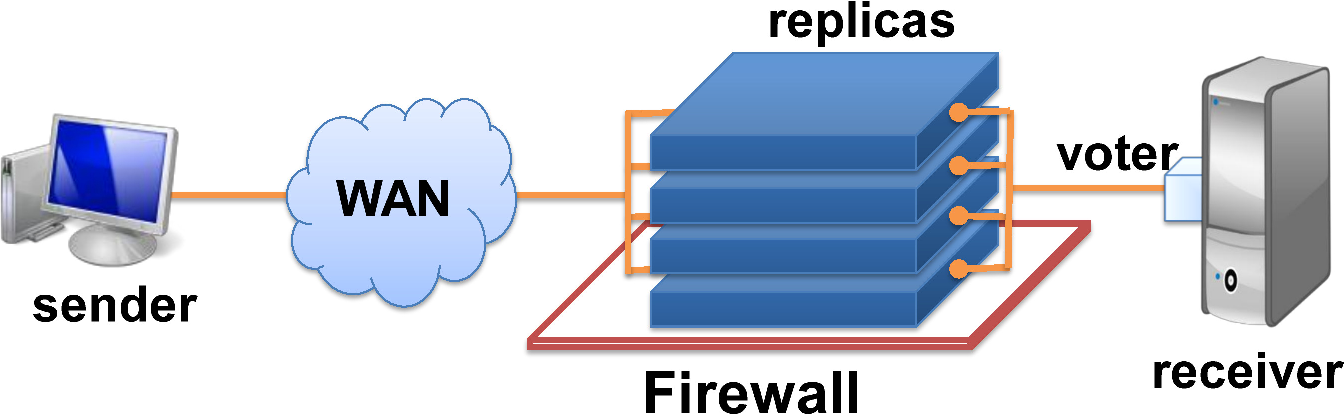
\includegraphics[width=.8\columnwidth]{images/images/arch_traditional.pdf}
\caption{Architecture of a state-of-the-art replicated firewall.}
\label{fig:traditional}
\end{center}
\end{figure}

Although this architecture has interesting characteristics, such as an increased failure resilience, it suffers from some fundamental limitations:

\begin{enumerate}

\item The dissemination of a message to all replicas can be detrimental to the proper operation of the firewall. 
For example, a traffic replicator device (e.g., hub) can be placed at the entry of the firewall to reproduce all messages~\cite{Sousa:2010,Roeder:2010} transparently. 
An obvious consequence of this approach is that malicious messages from an external attacker are also replicated, and therefore, all replicas have to spend the same effort to process them.
This result on attack amplification caused by the replicator device.
Alternatively, a leader replica could receive the traffic and then disseminate the messages to the others~\cite{Roeder:2010}.
The drawback is that the leader becomes a natural bottleneck, especially when under attack (instead of dispersing the attack load over all replicas~\cite{Amir:2011}).

\item The support for stateful firewall filtering requires that all correct replicas process messages in the same order~\cite{Schneider:1990}.
As a consequence, to ensure an agreement in a common sequence of messages, replicas need to continuously run a \gls{bft} consensus protocol~\cite{Castro:2002} to establish message ordering.
A significant amount of work can be wasted with malicious messages since all messages have to be agreed. This is particularly relevant because a consensus protocol consumes both computational and network resources.

\item The creation and check of the proof of validity can be a complex task. For example, one approach requires a trusted component to be deployed in the replicas to generate a \gls{mac} as a proof that a message is valid~\cite{Sousa:2010}. 
The component only returns the \gls{mac} when a quorum of replicas accepted the message. 
Another solution uses threshold cryptography to ensure that every replica can individually produce a partial signature (that corresponds to a part of the proof)~\cite{Roeder:2010}. 
To recreate the full proof, the voter needs to wait for the arrival of a quorum of partial proofs. 
When building a firewall, it would be useful if a more straightforward approach could be employed, with no need for specialized trusted components or expensive threshold cryptography.

\end{enumerate}

These drawbacks can have a significant impact on the firewall performance depending on the considered setting. 
For example, a typical \gls{dos} attack can create a substantial decrease in the throughput and several orders of magnitude growth in the latency of message delivery. 
To illustrate this behavior we implemented the architecture of Figure~\ref{fig:traditional} and launched a \gls{dos} attack on this system (see Section~\ref{evaluation} for a description of the setup and environment). 
The results show that the system performance is significantly affected by the attack (see Figure~\ref{fig:attack_traditional}).


\begin{figure}[h]
\begin{center}
\subfloat{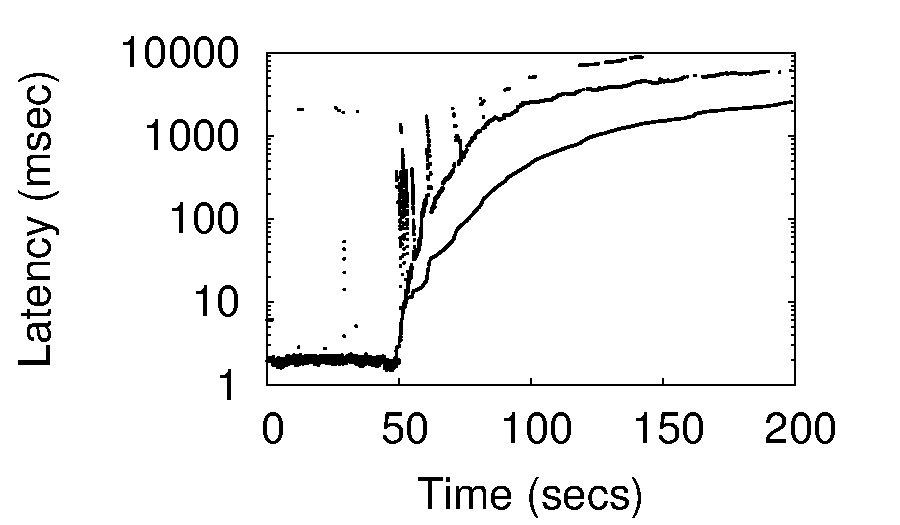
\includegraphics[width=0.5\columnwidth]{images/gnuplot/sieveq/plots/latency_tradiotional_attack.pdf}}
\hspace{-5mm}
\subfloat{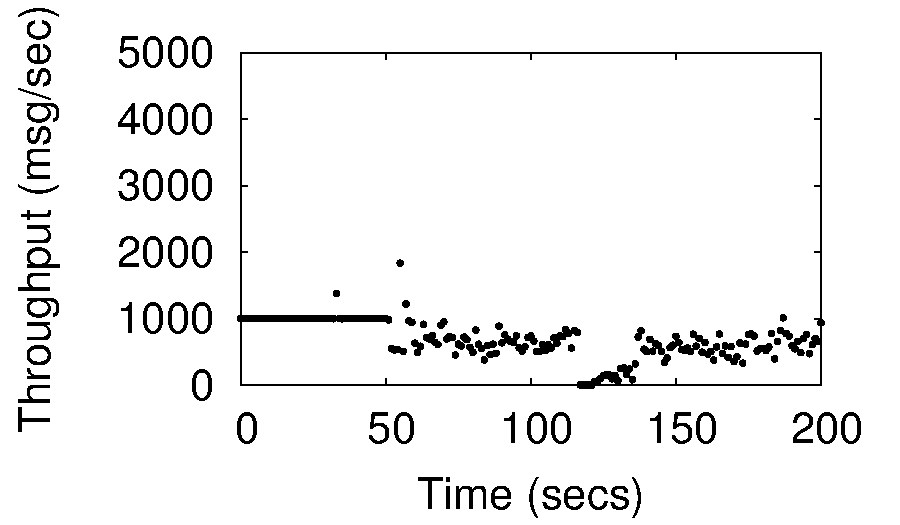
\includegraphics[width=0.5\columnwidth]{images/gnuplot/sieveq/plots/server_throughput_traditional_attack.pdf}}
\caption{Effect of a DoS attack (initiated at second 50) on the latency and throughput of the intrusion-tolerant firewall architecture displayed in Figure \ref{fig:traditional}.}
\label{fig:attack_traditional}
\end{center}
\end{figure}

In \sieveq, we explore a different design for replicated protection devices, where we trade some transparency on senders and receivers for a more efficient and resilient firewall solution.
In particular, we propose an architecture in which critical services and devices can only be accessed through a message queue and implement the application-level filtering in this queue.
It is assumed that these services have a limited number of senders, which can be appropriately configured to ensure that only they are authorized to communicate through \sieveq.

\section{Overview of \sieveq}
\label{architecture}

Typical resilient firewall designs are based on primary-backup replication, and consequently, they are able to tolerate only crash failures.
Therefore, more elaborated failure modes may allow an adversary to penetrate into the protected network.


Some organizations deal with crashes (or \gls{dos} attacks) by resorting to several firewalls to support multiple entry points. 
This solution is helpful to address some (accidental) failures, but is incapable of dealing with an intrusion in a firewall.
In this case, the adversary gains access to the internal network, enabling an escalation of the attack, which at that stage can only be stopped if other protection mechanisms are in place.

\sieveq provides a message queue abstraction for critical services, applying various filtering rules to determine if messages are allowed to go through.
\sieveq is not a conventional firewall and we do not claim that it should replace existing firewalls in all deployment scenarios.
We are focusing on service- or information-critical systems that require a high-level of protection, and therefore, justify the implementation of advanced replication mechanisms.
The system we propose is able to deliver messages while guaranteeing authenticity, integrity, and availability.
As a consequence, and in contrast to conventional firewalls, we lose transparency on senders and receivers, since they are aware of the \sieveq's end-points.
The rest of the section explains how we address some of the mentioned issues and introduces the main design choices and the architecture of \sieveq.

\subsection{Design Principles}
Our solution was guided by the following  principles:

\begin{itemize}

\item \emph{Application-level filtering}: support sophisticated firewall filtering rules that take advantage of application knowledge. \sieveq implements this sort of rules by maintaining state about the existing flows, and this state has to be consistently replicated using a \gls{bft} protocol.

\item \emph{Performance}: address the most probable attack scenarios with highly efficient approaches, and as early as possible in the filtering stages; Reduce communication costs with external senders, as these messages may have to travel over high latency links (e.g., do not require message multicasts).	

\item \emph{Resilience}: tolerate a broad range of failure scenarios, including malicious external/internal attackers, compromised authenticated senders, and intrusions in a subset of the \sieveq components; Prevent malicious external traffic from reaching the internal network by requiring explicit message authentication.

\end{itemize}

\subsection{\sieveq Architecture}

A fundamental difference of the \sieveq architecture, when compared with other replicated firewall designs (see Figure~\ref{fig:traditional}), is the separation of filtering in several stages.
The rationale for this change is to gain flexibility in the filtering operations while ensuring better performance under attack, retaining the ability to tolerate intrusions.
As observed previously, despite the significant improvements in state-of-the-art \gls{bft} implementations, there is an inherent trade-off between the benefits of \gls{bft} replication and its performance, namely due to the need to disseminate (and eventually authenticate) all messages at the replicas, which includes both valid and invalid messages.

Figure~\ref{fig:arch} presents the architecture of \sieveq. 
In this architecture, message processing starts with a first filtering layer that implements a message authentication mechanism and is responsible for discarding most of the malicious traffic efficiently. 
This layer is based on a set of \presieve modules, each of them in charge of the communications with a subgroup of senders. 
During a typical operation, a sender only interacts with its own \presieve.
The assignment of a \sender to a \presieve is done during the channel setup.
Initially, a sender connects with one of a few statically-configured \presieves.
If a \presieve becomes overloaded, it will request the creation of more \presieves (see details in Section~\ref{faultypresieve}) and/or hand of the new \sender channel to another node.

\begin{figure}[h]
\begin{center}
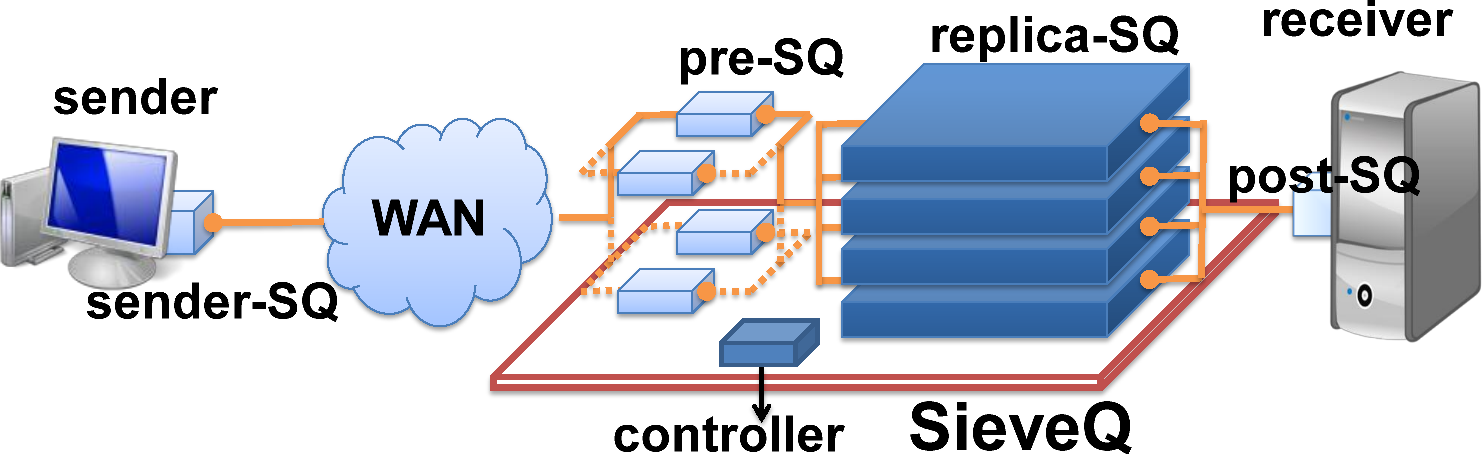
\includegraphics[width=0.9\columnwidth]{images/images/arch.pdf}
\caption{\sieveq layered architecture.}
\label{fig:arch}
\end{center}
\end{figure}

The messages are sent to the second filtering layer by the \presieve to perform a more detailed inspection, which can take advantage of state information kept from previous messages and application-related rules.
This layer is implemented by a group of \repsieves acting together as a \gls{bft} replicated state machine.
They receive all accepted messages from the \presieves and process them in the same order, which guarantees that every \repsieve reaches the same decision (discard or accept a message).
However, if $f$ replicas are faulty, their output could be different.
Consequently, as long as more than two-thirds of the \repsieves are correct, the right decision is taken by the \postsieve by performing a message voting.

In the following, we describe each module of \sieveq presented in Figure~\ref{fig:arch}:


\begin{itemize}

\item \sender: The sender nodes cooperate with \sieveq to secure the messages by deploying a \sender module locally. 
Its primary role is to secure the messages and assist in the detection of some intruded \sieveq components. 
The module can be implemented inside the sender's \gls{os} (e.g., as a kernel module or a specialized device driver) or as a library to be linked with the applications.
The decision to have this module corresponds to a trade-off in our design, where we are willing to lose some transparency to improve the system's resilience.

\item \presieve: These are the \sieveq front-end, and although it only performs stateless filtering to improve efficiency, it can deter the most common attacks. 
\Presieve modules discard invalid messages, while the approved ones are forwarded to the \repsieve using a \emph{Byzantine \gls{tom}} protocol~\cite{Bessani:2014}. 
The \presieves can be deployed, for instance, as \glspl{vm}. 
The effect of this layer is a significant reduction in the communication and computational overhead caused by malicious packets at the \repsieve.

\item \repsieve: These components implement a replicated filtering service that tolerates Byzantine faults. 
The actual filtering rules can be more or less complex depending on the needs of the critical service. 
The \gls{tom} ensures that \repsieves receive the messages in the same order. 
Consequently, identical rules are applied across the \repsieves, and therefore, the same decision should be reached on the validity of messages. 
Each \repsieve individually transmits approved messages to the final receiver (the others are dropped). 
Overall, this layer allows for sophisticated filtering as the replicas are stateful.

\item \postsieve: This module runs on the receiver side, and it is responsible for the delivery of messages to the application.
A \postsieve carries out a voting operation on the arriving data because a \repsieve might be intruded and corrupt messages.
It delivers a message to the application only after receiving the same approved message from a quorum of \repsieves.
From a deployment perspective, this module can be implemented in the \gls{os} or as a library, as in the sender.

\item \emph{controller}: This module is a trusted component of \sieveq that runs with high privilege.
It takes input from the \repsieves to decide on the creation or destruction of \presieves if some misbehavior is observed.
Depending on the actual \sieveq implementation, it can be developed in different ways.
This sort of component was used in previous works, and it can be implemented both in a centralized~\cite{Roeder:2010,Platania:2014} or distributed~\cite{Sousa:2010} way.
As already presented in Chapter~\ref{chap:lazarus_implementation}, we presented an implementation for this type of controllers.


\end{itemize}

\subsection{Resilience Mechanisms}

The \sieveq architecture is built to tolerate both faults with an accidental nature (e.g., crashes) and caused by malicious actions (e.g., a vulnerability is exploited and a specific module is compromised).
To be conservative, we assume that all failed components are controlled by a single entity, which will make them act together in the worst possible manner to defeat the correctness of the system. Therefore, failed components can for instance: stop sending messages, produce erroneous information, or try to delay the system. 
\sieveq performs several mitigation actions to guarantee a valid operation (as long as the number of faults is within the assumed bounds, see Section~\ref{fault_model}).

The most common attack scenario occurs when an external adversary attempts to attack a system that is being protected by \sieveq. 
He can deploy many nodes, whose aim is either to delay the communications or bypass \sieveq protection and reach the internal network. 
\sieveq addresses these attacks by discarding unauthenticated or corrupted messages with minimal effort at the \presieve filtering stage.
As with any other firewall, if a DoS attack completely overloads the incoming channels, \sieveq cannot handle or react to the attack.
The network needs to include other defense mechanisms to deal with this sort of problem~\cite{Mishra:2011}.

As (authenticated) senders  might be spread over many (outside) networks, it is advisable to consider a second scenario where an adversary is capable of taking control of some of these nodes. 
In this case, we assume that the adversary gains access to all data stored locally, including the \sender keys. 
Thus, he will be able to generate traffic that is correctly authenticated, allowing these messages to go through the first filtering step.
The messages are however still checked against the application related rules (namely, the ones defined in the \repsieve), which can cause most malicious traffic to be dropped (e.g., a pre-defined \sender can only send messages to a particular \postsieve accordingly to a specific application protocol).
If the messages follow all the rules, the firewall has to forward them because they are indistinguishable from any other valid messages.

A third scenario occurs when the adversary is able to cause an intrusion in \sieveq and compromises a few of the \presieves and/or \repsieves. 
When this happens, these components can act in an erroneous (Byzantine) way. 
However, unlike with an intruded \sender, malicious \presieves cannot generate fully authenticated messages, since they lack all the required keys. 
They can still perform \gls{dos} attacks on the \repsieves, e.g., by transmitting many messages, but this strategy creates an obvious misbehavior allowing immediate discovery. 
Malicious \presieves are detected with the assistance of correct \sender and  \repsieves, eventually leading to their substitution.

\Repsieves modules are much harder to exploit because they do not face the external network. However, if they end up being intruded, \repsieves can produce arbitrary traffic to the internal network. \Postsieve addresses this issue by carrying out a voting step, which excludes these messages. Moreover, an alarm is generated and sent to the \emph{controller}.

The \sieveq architecture makes no attempt to recover from intrusions in the \emph{controller} and \postsieve.
The first is assumed to be trusted, as it is deployed in a separated administrative domain and is to be used only in a few very specific operations.
Moreover, its simplicity allows the audit of its code and ensures correctness with a high level of confidence.
The \postsieve already runs in the internal network, and therefore, \sieveq can not preclude its misbehavior.



\subsection{System and Threat Model}
\label{fault_model}

The system is composed of a (potentially) large number of external nodes, called \emph{senders}, some internal nodes, called \emph{receivers}, and \sieveq nodes.
Senders run \sender modules to be able to transmit packets through the \sieveq, while receivers receive validated messages by using \postsieve modules. 

Communications can experience accidental faults or attacks.
Thus, packets might be lost, delayed, reordered or corrupted, but we assume that if messages are retransmitted, eventually they will be correctly received by \sieveq.
The fault model also assumes that \sender, \presieve, and \repsieve nodes can suffer from arbitrary (Byzantine) faults.
When this happens, failed nodes may perform actions that deviate from their specification, including colluding against the system.
However, at most $f_{ps}$ \presieves from a total of $N_{ps} = f_{ps} + k$ (with $k > 1$), and $f_{rs}$ \repsieve from a total of $N_{rs} = 3f_{rs}+1$ may fail.
Redundant components should fail independently by employing diversity techniques such as the ones described in Chapter~\ref{chap:lazarus_design}.
A component that is unable to communicate is also considered faulty because from a practical perspective it is indistinguishable from a crashed module.

The cryptographic operations used in the \sieveq protocol are assumed to be secure, and therefore, they cannot be subverted by an adversary. 
Consequently, traditional properties of digital signatures, \glspl{mac}, and hash functions will hold as long as the associated keys are kept safe.
The deployment of \sieveq requires a key distribution scheme to create shared keys between the \sender and the \presieve and to periodically re-issue private-public key pairs for the \sender.
We assume that the key distribution scheme is similar to solutions that already address this sort of problem (e.g.,~\cite{Harkins:1998}).
If required, the key distribution infrastructure could also be made intrusion-tolerant~\cite{Kreutz:2014,Zhou:2002}.


\subsection{Resilience Mechanisms}


The \sieveq architecture is built to tolerate both faults with an accidental nature (e.g., crashes) and caused by malicious actions (e.g., a vulnerability is exploited, and a specific module is compromised).
To be conservative, we assume that all failed components are controlled by a single entity, which will make them act together in the worst possible manner to defeat the correctness of the system. Therefore, failed components can stop sending messages, produce erroneous information, or try to delay the system. 
\sieveq performs several mitigation actions to guarantee a valid operation (as long as the number of faults is within the assumed bounds, see Section~\ref{fault_model}).



The most common attack scenario occurs when an external adversary attempts to attack a system that is being protected by \sieveq. 
He can deploy many nodes, whose aim is either to delay the communications or bypass \sieveq protection and reach the internal network. \sieveq addresses these attacks by discarding unauthenticated or corrupted messages with minimal effort at the \presieve filtering stage.
As with any other firewall, if a \gls{dos} attack completely overloads the incoming channels, \sieveq cannot handle or react to the attack.
The network needs to include other defense mechanisms to deal with this sort of problem~\cite{Mishra:2011}.

As (authenticated) senders might be spread over many (outside) networks, it is advisable to consider a second scenario where an adversary is capable of taking control of some of these nodes. 
In this case, we assume that the adversary gains access to all data stored locally, including the \sender keys. 
Thus, he will be able to generate traffic that is correctly authenticated, allowing these messages to go through the first filtering step.
Then, the messages are still checked against the application related rules (namely, the ones defined in the \repsieve), which can cause most malicious traffic to be dropped (e.g., a pre-defined \sender can only send messages to a particular \postsieve accordingly to a specific application protocol).
If the messages follow all the rules, the firewall has to forward them because they are indistinguishable from any other valid messages.


A third scenario occurs when the adversary can cause an intrusion in \sieveq and compromises a few of the \presieves and/or \repsieves. 
When this happens, these components can act in an erroneous (Byzantine) way. 
However, unlike with an intruded \sender, malicious \presieves cannot generate fully authenticated messages, since they lack all the required keys. 
They can still perform \gls{dos} attacks on the \repsieves, e.g., by transmitting many messages, but this strategy creates apparent misbehavior allowing immediate discovery. 
Malicious \presieves are detected with the assistance of correct \sender and \repsieves, eventually leading to their substitution.

\Repsieves modules are much harder to exploit because they do not face the external network. 
However, if they end up being intruded, \repsieves can produce arbitrary traffic to the internal network. 
\Postsieve addresses this issue by carrying out a voting step, which excludes these messages. Moreover, an alarm is generated and sent to the \emph{controller}.

The \sieveq architecture does not attempt to recover from intrusions in the \emph{controller} and \postsieve.
The \postsieve already runs in the internal network, and therefore, \sieveq can not preclude its misbehavior.
In this chapter the \emph{controller} is assumed to be trusted, as it is deployed in a separated administrative domain and is to be used only in a few particular operations.
Moreover, its simplicity allows the audit of its code and ensures correctness with a high level of confidence.


\section{\sieveq Protocol}
\label{protocol}


This section details the \sieveq protocol and the service properties. 
We conclude the section with an analysis of the behavior of the system under different kinds of attacks and component failures, and highlight how the countermeasures integrated in our design mitigate such threats.

\subsection{Properties}
\label{properties}

\sieveq protocol guarantees the following three properties for messages transmitted from a sender to a receiver:

\begin{security}
If a message, transmitted by a correct sender, is delivered to a correct receiver then the message is in accordance with the security policy of \sieveq.
\end{security}

\begin{validity}
If a correct receiver delivers a message \msg.\texttt{DATA}, then the message was transmitted by \msg.\texttt{sender}.
\end{validity}

\begin{liveness}
If a correct sender sends a message, then the message eventually will be delivered to the correct receiver.
\end{liveness}

These properties require \sieveq to behave in a way similar to most firewalls while offering a few extra guarantees. 
Only external messages that are approved by the policies defined in \sieveq can reach the receivers, and the rest should be dropped (Compliance). 
\Postsieve can use the message field \msg.\texttt{sender} to find who transmitted the message contents (\msg.\texttt{DATA}), and accordingly decide if the message should be delivered to the receiver application (Validity). 
Progress is also ensured, as correct senders eventually can transmit their messages (Liveness).

Besides these functional properties (related to message filtering), \sieveq also ensures a \emph{resilience} property related to the detection and recovery of components of the system that exhibit faulty behavior:


\begin{resilience}
Every component exhibiting observable faulty behavior will be eventually removed or recovered.
\end{resilience}

In the following we present the mechanisms for implementing the \sieveq functionalities, i.e., the mechanisms for satisfying the three functional properties stated above.
The mechanisms for ensuring resilience will be detailed after that.

\subsection{Message Transmission}
\label{transmittingmessage}


\paragraph{\Sender processing}

This module gets a buffer with the \texttt{DATA} to be transmitted to a particular application placed behind \sieveq.
The buffer needs to be encapsulated in a message with some extra information required for protection (see (\ref{msg}), below): we add a \sender identifier $\senderi_i$ and a sequence number \sn that is incremented on each message.
This information is needed to prevent replay attacks, either from the network or from a compromised \presieve.
Some information is also added to protect the integrity and authenticate the message.
A signature $\signature_{Si}$ is performed over the message contents, and a \gls{mac} $\mac_{ski}$ is computed using a shared key established with the \presieve.
This \gls{mac} serves as an optimization to speed up checks~\cite{Clement:2009}.

\begin{equation}
\msg = \langle \senderi_i, \sn, \texttt{DATA}, \signature_{Si} \rangle_{\mac_{ski}}
\label{msg}
\end{equation}

\begin{figure}[!t]
\centering
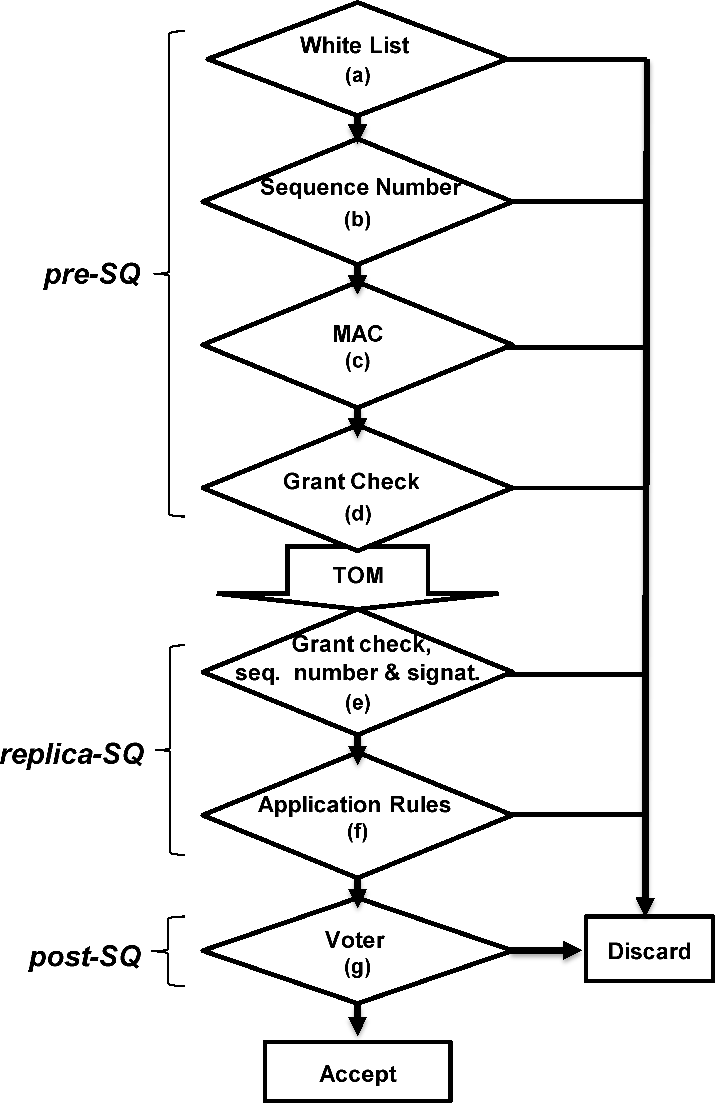
\includegraphics[scale=0.5]{images/images/filtering_steps_1.pdf}
\caption{Filtering stages at the \sieveq.}
\label{fig:filters}
\end{figure}


After constructing the message, it is sent to the \presieve assigned to the \sender, and a timer is started.
If this timer expires before the \sender receives an acknowledgement message, it re-sends the \msg to another \presieve.

\paragraph{\Presieve filtering}

The \presieve determines if an arriving message \msg should be forwarded or discarded (stages (a)--(d) in Figure~\ref{fig:filters}). It applies the following checks to make this decision:

\begin{enumerate}

\item[(a)] \textbf{White list:} each \presieve maintains a list of the nodes that are allowed to transmit messages (i.e., which were authorized by the system administrator). 
Messages coming from other nodes are dropped.
This check is based on the address of the message sender, and therefore it serves as an efficient first test, but it is vulnerable to spoofing.

\item[(b)]  \textbf{Sequence number:} finds out if a message with sequence number \sn from \sender $\senderi_i$ was seen before.
In the affirmative case, the message is discarded to prevent replay attacks.
Messages are also dropped if their \sn is much higher than the largest sequence number ever observed from that \sender (a sliding window of acceptable sequence numbers is used).

\item[(c)]  \textbf{MAC test:} \gls{mac} $\mac_{ski}$ is verified to authenticate the message contents, including to find out if the expected $\senderi_i$  is the sender. 
If the check is invalid, the message is dropped, and the sequence number information is updated to forget that this message was ever received (the update carried out in the previous step needs to be undone).

\item[(d)] \textbf{Grant check:} each \presieve controls the amount of traffic that a \sender is transmitting.
Messages that fall outside the allocated amount are dropped to ensure that all senders get a fair share of the available bandwidth (and to avoid \gls{dos} attacks by compromised senders).
The amount of traffic that is allowed to each \sender is adjusted dynamically based on the available and consumed resources.


\end{enumerate}

Finally, the \presieve invokes the \gls{tom} primitive to forward the message to every correct \repsieve.

\paragraph{\Repsieve filtering}
When a correct \repsieve delivers a message to be filtered, the following checks are applied:

\begin{enumerate}
\item[(e)] \textbf{Grant check, sequence number, and signature:} since a \presieve may have been intruded and may collude with malicious \sender, extra checks are required on the amount of forwarded traffic and on the integrity of the message.
The grant check and the test on the sequence number are similar to the ones performed by the \presieve, and the signature ensures that all \repsieves reach the same decision regarding the validity of the message content.
\item[(f)] \textbf{Application-level rules:} apply the application-defined filtering rules to determine if the message is compliant with the security policy of the firewall.
\end{enumerate}

Although uncommon, it can happen that \repsieves receive messages in a different order from what is defined in their sequence numbers.
As a consequence, the \repsieve's application-level rules may drop some of the out-of-order messages, which later on will have to be re-transmitted by the \sender.
For example, if messages \texttt{A} and \texttt{B} should appear in this sequence but are re-ordered, then the rules may consider \texttt{B} invalid and then accept \texttt{A}.
At some point, the \sender would consider \texttt{B} as lost, and re-transmit it.\footnote{It is important to remark that, independently of any violation on the order of delivery of sender messages, all correct \repsieves receive the messages in the same order.}

To address this issue, each \repsieve enqueues messages with a sequence number greater than the expected for a while, as long as they do not exceed a threshold above the last processed sequence number. These messages are processed when either: 1) the missing messages with smaller sequence numbers arrive, and then they are all tested in order, or 2) the \repsieve gives up on waiting, and checks the enqueued messages. This last decision is made after processing a pre-determined number of other messages.

Valid messages are encapsulated in a new format (see (\ref{msgl}), below) and are sent to their receivers.
Basically, \repsieve $\replicak_j$ substitutes the signature with a new \gls{mac}, $\mac_{skj}$.
This \gls{mac} is created with a shared key between the \repsieve and the \postsieve.

\begin{equation}
\msg' = \langle \senderi_i, \sn, \texttt{DATA}, \replicak_j \rangle_{\mac_{skj}}
\label{msgl}
\end{equation}

\paragraph{\Postsieve processing}

\Postsieve accumulates the messages that arrive from \repsieves until enough evidence is collected to allow their delivery.

\begin{enumerate}
\item[(g)] \textit{vote:} A message can be delivered to the application when it is received from $f_{rs} + 1$ \repsieves.

\end{enumerate}

Algorithm \ref{algo:post_filter} presents the \postsieve voting protocol.
The \postsieve starts by checking if the message contains a valid \gls{mac} (lines 5 and 6).
Then, it finds out if the message carries an acceptable sequence number before storing it in a \texttt{WaitingQuorom} set (lines 7 and 8).
Notice that a different set is used for each sender $S_i$ and $sn$ pair.
Messages with sequence numbers already delivered or higher than a threshold (\texttt{snThreshold}) are discarded.

The expected sequence number is stored in the auxiliary variable $k$ (line 9).
Next, the \postsieve tries to find a message with this sequence number and with at least $f_{rs} + 1$ votes (by searching the corresponding set and using function \texttt{equalMsg} --- line 10).
For each different \texttt{DATA} value that may exist in the set, the \texttt{equalMsg} function counts the number of times its appears, and returns the largest count.\footnote{Notice that all correct \repsieves transmit messages with the same \texttt{DATA} value and that malicious replicas can send at most $f_{rs}$ arbitrary \texttt{DATA} values.
Therefore, eventually there will be a \texttt{DATA} value with at least $f_{rs}+1$ votes because there are at least $2f_{rs}+1$ correct \repsieves.}
Next, while there are \msg's with a $f_{rs} + 1$ quorum, \postsieve delivers \msg's in order (line 10-13).
The function \texttt{mostVotedMsg} returns the message with the \texttt{DATA} value with most votes (line 11).
Then, the \texttt{deliver} function delivers \texttt{DATA} to the application on the receiver and deletes the \texttt{WaitingQuorom} set.
Finally, the \texttt{snExpect} is incremented (line 12) and the $k$ index is updated (line 13).
This allows \postsieve to deliver messages in order while there are messages with the expected sequence number in its buffer.

\SetKwInOut{Input}{input}
\SetKwData{repsievealgo}{\repsieve}

\SetKwData{MAC}{$\mac_{si}$}
\SetKwData{Signature}{\signature}
\SetKwData{SeqNumber}{\texttt{\sn}}
\SetKwData{SeqNumberExp}{\texttt{snExpect}}
\SetKwData{SeqNumberThreshold}{\texttt{snThreshold}}
\SetKwData{MESSAGE}{\msg}
\SetKwData{MESSAGEX}{\texttt{aux}}
\SetKwData{DATA}{\texttt{DATA}}

\SetKwData{client}{\senderi$_{i}$}
\SetKwData{prefirewall}{\presieve\emph{$_{i}$}}
\SetKwData{prefirewalltwo}{\presieve\emph{$_{k}$}}
\SetKwData{RepFirewallID}{\repsieve\emph{$_{i}$}}
\SetKwData{WaitingQuorom}{WaitingQuorom}

\SetKwFunction{seqnumber}{expected\_seq\_numb}
\SetKwFunction{macverification}{verifyMAC}
\SetKwFunction{sendVoter}{send\_\postsieve}
\SetKwFunction{applicationRules}{application\_rules}
\SetKwFunction{discard}{discard}
\SetKwFunction{deliver}{deliver\_to\_Application}
\SetKwFunction{existsQuorom}{existsQuorom}
\SetKwFunction{deliver}{deliver}
\SetKwFunction{return}{return}
\SetKwFunction{equalMsg}{equalMsg}
\SetKwFunction{mostVotedMsg}{mostVotedMsg}

{\centering
\begin{minipage}{.7\linewidth}
 
\begin{algorithm}[H]
\caption{\postsieve protocol}\label{algo:post_filter}
{
\footnotesize

  $Init:\ executed\ only\ once$\\
	$\SeqNumberExp_{Si}, k \leftarrow 0$\;
	$\WaitingQuorom_{Si,\sn} \leftarrow \perp$\;
  \BlankLine
\Fn{Filter (\MESSAGE')}{
    \If{( \macverification{\MESSAGE'} = FALSE )}{
        \return $errorMAC$\;
    }
	\If{ ($\SeqNumberExp_{Si}$ $\leq$ \MESSAGE'.\SeqNumber $<$ ($\SeqNumberExp_{Si}$ + \SeqNumberThreshold)) }{
		$\WaitingQuorom_{Si,\sn} \leftarrow \WaitingQuorom_{Si,\sn} \cup \{ \MESSAGE' \}$\;
	}
	$k \leftarrow \SeqNumberExp_{Si}$\;



	\While{ ( \equalMsg{$\WaitingQuorom_{Si,k}$} $\geq$ $f_{rs}+1$ ) }{

		  	\deliver{\mostVotedMsg{$\WaitingQuorom_{Si,k}$}} \;
		  	$\SeqNumberExp_{Si} \leftarrow \SeqNumberExp_{Si} + 1$ \;
			$k \leftarrow \SeqNumberExp_{Si}$\;

    }
}
}
\end{algorithm}
\end{minipage}
\par
}





\subsubsection{Correctness Argument}
In the following, we show that \sieveq design satisfies the three functional properties described in Section~\ref{properties}.
The proofs work under the assumptions of our system and threat model (defined in Section~\ref{fault_model}).

\begin{validity}

If a correct receiver delivers a message \msg.\texttt{DATA}, then the message was transmitted by \msg.\texttt{sender}.
\end{validity}

\begin{proof}
Assume that a receiver $\receiverj_j$ gets a message content \msg.\texttt{DATA} with the \msg.\texttt{sender} $=$ \msg.\texttt{$\senderi_i$}.
For this to happen, the \postsieve of $\receiverj_j$ waited for the arrival of at least $f_{rs}+1$ correctly authenticated messages\footnote{Note that \repsieves send $\msg'$ (defined in (\ref{msgl}))  instead of \msg (defined in (\ref{msg})). Both are similar, but \msg' has a \gls{mac} instead of a signature to authenticate its contents with \postsieve (see Section~\ref{sec:repseivefiltering}). For the sake of simplicity we will only use the $\msg$ notation in the rest of the proof.} with equal \msg.\texttt{$\senderi_i$}, \msg.$\sn$, and \msg.\texttt{DATA}.
Therefore, at least $f_{rs}+1$ \repsieves received $\msg$ signed by $\senderi_i$, and verified the signature $\signature_{Si}$ as valid.
This indicates that \msg.\texttt{DATA} was not modified by the network or by any \presieve.
Only a sender \msg.\texttt{$\senderi_i$} (correct or not) can create and authenticate a $\msg$ with its signature.
Therefore, $\senderi_i$ is the \msg.\texttt{sender}, i.e., the creator of \msg.\texttt{DATA}.
\end{proof}


\begin{security}
If a message, transmitted by a correct sender, is delivered to a correct receiver then the message is in accordance with the security policy of \sieveq.
\end{security}


\begin{proof}
The proof of the \emph{Compliance} property is very similar to the \emph{Validity} proof.
The difference is that, we also know that if $f_{rs}+1$ \repsieves sent $\msg$ to a \postsieve, then $\msg$ was verified against the security policy in at least one correct \repsieve, which approved it.
\end{proof}



\begin{liveness}
If a correct sender sends a message, then the message eventually will be delivered to the correct receiver.
\end{liveness}

\begin{proof}
For the sake of simplicity, our proof only considers nodes that drop or delay messages.
Attacks to the integrity will make the message be discarded (i.e., dropped).

Assume that a sender $\senderi_i$ transmits a message $\msg$ with the sequence number $\sn$ to a \presieve $\presievei_u$.
Then $\senderi_i$ sets a timer $timer_{sn}$ for \msg.\sn.
If $\presievei_u$ is correct, after it receives a message, it re-sends $\msg$ via \gls{tom} to the \repsieves.
At least $f_{rs}+1$ correct \repsieves will send $\msg$ to the \postsieve, which will deliver  \msg.\texttt{DATA} to the receiver $\receiverj_j$.
If the $\presievei_u$ is faulty, i.e., drops or delays messages, $timer_{sn}$ in $\senderi_i$ will eventually expire.
When this happens, $\senderi_i$ re-transmits $\msg$ to another \presieve.
Eventually, this process will make some correct \presieve forward $\msg$ to the \repsieves using the \gls{tom} primitive, which will cause \msg.\texttt{DATA} to be delivered to $\receiverj_j$.
\end{proof}


\subsection{Addressing Component Failures}
\label{sec:failures}

In this section, we discuss the implications of failures in the different components of the \sieveq, and how they are handled for ensuring the \emph{Resilience} property stated in Section~\ref{properties}.

In the Byzantine model, every failed component can behave arbitrarily, intentionally or accidentally. Therefore, the \sieveq design incorporates mechanisms that are resilient to different failure scenarios. 
Given the architecture of Figure~\ref{fig:arch}, one has to address faults in authenticated \senders, \presieves and \repsieves, as they are the main components subject to Byzantine failures in our model. 
\Postsieve is not considered in this section as it is co-located with the receiver.
Therefore, we can not make further assumptions on it. 
In this chapter, we assume the \emph{controller} as trusted for simplicity.
In Chapter~\ref{chap:lazarus_implementation} we presented an intrusion-tolerant \emph{controller}


In the following, we try to focus on complex scenarios in whereas faulty components send syntactically-valid messages. Therefore avoiding cases that could be easily detected and recovered by existing network monitoring and protection tools (e.g., it is easy to discover that a \presieve is sending messages to another \presieve, something our protocol does not allow).

Since \presieves are directly exposed to the external network, there is a higher risk of them being compromised.
Then, to keep the \sieveq operational, it is required that failed \presieves are identified and recovered.
We leverage from the \repsieve setup to perform failure detection, and then use the \emph{controller} to restart erroneous \presieves.
Replacing these components is almost trivial because they are stateless.

\Repsieves execute as a \gls{bft} replicated state machine, processing messages in the same order and producing identical results.
Consequently, \repsieves faults can be tolerated by employing a voting technique on the \postsieve that selects results supported by a sufficiently large quorum (as explained above, an output with at least $f_{rs} + 1$ votes).
Below, we discuss in more detail a few failure scenarios.



\subsubsection{Faulty \Sender}


A faulty \sender is authorized to communicate while suffering from some arbitrary problem (e.g., intrusion). 
Therefore, it can produce correctly authenticated messages to attack the firewall. 
In some scenarios, it is possible to discard these messages. 
For example, if the \sieveq receives a correctly signed message with a sequence number is higher than what was expected, then it can be easily detected and eliminated (checks \emph{(b)} and \emph{(e)} in Figure~\ref{fig:filters}).

A more demanding scenario occurs when a \sender transmits faster than the allowed rate (verification (d) of Figure~\ref{fig:filters}).
In this case, some defense action has to be carried out, as these attacks can lead \sieveq to waste resources.
To be conservative, we decided to follow a simple procedure to protect the firewall: \sieveq maintains a counter per sender that is incremented whenever new evidence of failure can be attributed to it, e.g., the faulty \sender is overloading the system with invalid messages or if it is sending messages to \presieves which it was not assigned.
When the counter reaches a pre-defined value, the \sender is disallowed from communicating with \sieveq by temporarily removing it from the whitelist and adding it to a quarantine list (failing verification (a) of Figure~\ref{fig:filters}) and by giving a warning to the system administrator.
\emph{This ensures that faulty \emph{\senders} are eventually removed from the system.}

Excluded \senders may regain access to the service later on because the counter is periodically decreased (when the counter falls below a certain threshold, the \sender is moved back into the whitelist). 
Additionally, the administrator is free to update the white/quarantine lists. 
For instance, he may choose to manually add a faulty sender to the quarantine list or even deploy policies to do that under certain conditions (e.g., if the same sender is in the quarantine list for a certain number of times).


\subsubsection{Faulty \Presieve}
\label{faultypresieve}


Addressing failures in \presieves is difficult because these components may look as compromised even when they are correct.
Notably, when a \presieve is under a \gls{dos} attack, messages can start to be dropped due to buffer exhaustion, and this is indistinguishable from malicious behavior in which messages are selectively discarded.
In the same way, a failed signature check at a \repsieve indicates that either the \presieve is faulty (it is tampering/generating invalid messages) or that a \sender is misbehaving (recall that a \presieve verifies the message \gls{mac}, but not its signature).
Finally, a \repsieve may also detect problems if it observes a sudden increase in the arrival of messages (above the grant check), which could indicate a \gls{dos} attack by a malicious \presieve (maybe colluding with a compromised \sender).
This kind of ambiguity precludes exact failure detection, and consequently, we aim to provide a mechanism that allows \sieveq to recover from end-to-end problems and continue to deliver a correct service.

An initial step to deal with these complex failure scenarios is to make \presieves evaluate their own state.
This is done by analyzing the amount of arriving traffic and by observing if it could overload the \presieve.
The analysis can be done by measuring the inter-arrival times of messages over a specified period.
If those intervals are small (on average), there is a chance that the \presieve is working at its full capacity or is even overloaded.
When this happens, the \presieve broadcasts (using the \gls{tom} primitive) a \texttt{WARNREQ} message to the \repsieves, so that they may take some action to solve the problem (see below).


When the \presieve is faulty, the \sender and \repsieves need to detect it together.
\sieveq provides a procedure to find how many messages are being discarded on \presieve:


\begin{enumerate}

\item Periodically, the \sender sends a special \texttt{ACKREQ} request to \repsieves, in which it indicates the sequence number of the last message that was sent (plus a signature and a \gls{mac}).
This request is first sent to the preferred \presieve, but if no answer is received within some time window, and then it is forwarded to another \presieve.
The waiting period is adjusted in each retransmission by doubling its value.

\item When the \repsieves receive the request, the included sequence number together with local information are used to find how many messages are missing. 
The local information is the set of sequence numbers of the messages that were correctly delivered since the last \texttt{ACKREQ}.

\item Based on the number of missing messages, the \repsieves transmit through the same \presieve a response \texttt{ACKRES} to the sender, where they state the observed failure rate and other control information (plus a signature).
\Repsieves may also perform some recovery action if the failure rate is too high.

\end{enumerate}

Additionally, if a \repsieve detects that a signature is invalid or that it is receiving more messages than the expected (check (e) in Figure \ref{fig:filters}), it suspects the \presieve that sent the messages and takes some action.


Once the problem is detected, the \repsieves should attempt to fix the erroneous behavior by employing one of three possible remediation actions, depending on the extent of the perceived failures:

\begin{itemize}


\item \emph{Redistribute load:} if a \presieve has sent a warning about its load, or a high failure rate related with this component is observed, the first course of action is to move some of the messages flows from the problematic component to other \presieve.
This is achieved by specifying, in the \texttt{ACKRES} response to a \sender, the identifier of a new \presieve that should be contacted.
At that point, the \sender is expected to connect to the indicated \presieve and begin sending its traffic through it.

\item \emph{Increase the \emph{\presieves} capacity:} if the existing \presieves are unable to process the current load, then the \sieveq needs to create more \presieves (depending on the available hardware resources).
To do that, \repsieves contact the \emph{controller} informing that an extra \presieve should be started.
When the controller receives $f_{rs} + 1$ messages, it performs the necessary steps to launch the new \presieve (which are dependent on the deployment environment).
The new \presieve begins with a few startup operations, which include the creation of a communication endpoint, and then it uses the \gls{tom} channel to inform the \repsieve that it is ready to accept messages from \senders.

\item \emph{Kill the \emph{\presieve}:} when there is a significant level of suspicion on a \presieve, the safest course of action is for \repsieves to ask the controller to destroy it.
Moreover, if the load on the firewall is perceived as having decreased substantially, the \repsieves select the oldest \presieve for elimination, allowing eventual aging problems to be addressed.
The controller carries out the needed actions when it gets $f_{rs} + 1$ of such requests (once again, which depend on how \sieveq is deployed).
The affected \senders will be informed about the \presieve replacement through the \texttt{ACKREQ} mechanism, i.e., they will eventually use another \presieve to send a request, and get the information about their newly assigned \presieve in the response.
Moreover, the new \presieve is informed about the expected sequence number for each \sender.
This information is stored by \repsieves, which contrary to \presieves are stateful.

\end{itemize}

Together, these mechanisms ensure that \emph{a faulty \emph{\presieve} affecting the \sieveq performance will be eventually removed from the system}.


\subsubsection{Faulty \Repsieve}
\label{faultyrepsieve}

A \postsieve only delivers a message if it receives $f_{rs}+1$ matching approvals for this message.
Given the number of \repsieves, this quorum is achievable for a correct message even if up to $f_{rs}$ \repsieves are faulty.
However, a faulty \repsieve can create a large number of messages addressed to other components of the system, effectively causing a \gls{dos} attack.
Therefore, we need countermeasures to disallow a faulty \repsieve to degrade the performance of the system in a similar way as illustrated in Figure~\ref{fig:attack_traditional}.
For example, a faulty \repsieve can send an unexpected amount of messages to a \presieve, making it slower and triggering suspicions that may lead it to be killed.
Similarly, it can attack other \repsieves to make the system slower.
Finally, a faulty \repsieve can also overload the \postsieve with invalid messages.

Each of these attacks requires a different detection and recovery strategy:

\begin{itemize}

\item When a \presieve is being attacked it complains to the controller, which first requests the \presieve replacement (assuming it might be compromised) and increases a suspect counter against the \repsieve.
If $f_{ps}+1$ \presieves also complain about the same \repsieve, the controller starts an \emph{individual recovery} in this \repsieve (see below).

\item If more than $f_{rs}$ other \repsieves are being attacked, they will probably become slower.
In this case, it is possible to detect such attacks if $f_{rs}+1$ \repsieves complain about a single \repsieve.
This would be possible because target \repsieves would observe unjustifiable high traffic coming from a single replica and because such spontaneously generated messages would be deemed invalid.
When this attack is detected, the controller starts an individual \repsieve recovery.

\item If only up to $f_{rs}$ other \repsieves are being attacked it is still possible to make the system slower without being detected by the previous mechanism.
This happens because $N_{rs}-f_{rs}$ replicas must participate in the \gls{tom} protocol~\cite{Bessani:2014}, and the target $f_{rs}$ plus the attacker intersect this quorum in a least one component. 
This intersecting component will define the pace of the messages coming, which typically will be slow.
We can mitigate this attack as each \repsieve periodically informs the \postsieve about its throughput (number of processed messages per second), piggybacking this value in some approved messages submitted for voting.
The \postsieve verifies that there are \repsieves presenting throughputs lower than expected and initiates a \emph{recovery round} on all the \repsieves (as described below).

\item When the \postsieve is being attacked it detects the abnormal behavior.
Then, it requests the individual recovery of the compromised replica.

\end{itemize}

The previous mitigation mechanisms suggest two kinds of recovery actions.
First, an individual recovery, where the machine is rebooted with clean code (we addressed this in Chapter~\ref{chap:lazarus_design}) and then is reintegrated in the system.
Second, a recovery round is used when a performance degradation attack is detected, but there is no certainty about which \repsieve was compromised.
%Therefore, in this case, we recover all replicas, one after another to avoid unavailability periods in the system, just like in proactive recovery systems~\cite{Castro:2002,Sousa:2010,Roeder:2010}.
%There are several works that present these techniques, and most of them are compatible with our architecture, therefore we refrain from describing them in more detail.
%Notice that the use of a recovery round is enough to ensure that \emph{a faulty \emph{\repsieve} will eventually be recovered in \sieveq}.

The integration of these reactive recovery mechanisms into \system' risk management can be assessed by drastically increasing the an individual risk of each replica (e.g., similarly to the \emph{age} value of reach replica). 
Then, \system proceed on the recovery of the faulty replica.


\section{Implementation}
\label{implementation}


We implemented a prototype of \sieveq following the specification of the previous section to validate our design.
The \sender and \postsieve were developed as libraries that are linked with the sender and receiver applications. 
The libraries offer an interface similar to the \gls{tcp} sockets, to simplify the integration and minimize changes both in the client and server applications. 
A sender can provide a buffer to be transmitted, and the receiver can indicate a buffer where the received data is to be stored.
Internally, the \sender library adds a \gls{mac} and a signature to each message. 
The \gls{mac} is created using \gls{hmac} with the \gls{sha}-256 hash function and a 256-bit key, and the signature employs \gls{rsa} with 512-bit keys. 
Messages are authenticated at the \postsieve also using \gls{hmac}. 
The \gls{rsa} keys were kept relatively small for performance reasons. 
However, since they should be updated periodically (e.g., every few hours), this precludes all practical brute force attacks~\cite{David:2015}.%%%%%%%%%%%%%%%%%%%%%%%%%%%%%%%%%

The \presieves operate as separate processes receiving the messages and forwarding them to the \repsieves.
We resorted to BFT-SMaRt, a \gls{smr} library~\cite{Bessani:2014}, to implement the \gls{tom} and manage the \repsieves.
BFT-SMaRt, like most \gls{smr} systems (e.g., PBFT~\cite{Castro:2002}, Zyzzyva~\cite{Kotla:2010}, Prime~\cite{Amir:2011}) follows a client-server model, where a client transmits request messages to a group of server replicas and then receives the output messages with the results of some computation.
We had to modify BFT-SMaRt because this model does not fit well with the message flow of \sieveq.
Therefore, we have decoupled the client-server model into a client-server-client model.
The client sends messages (but does not wait for responses as in the traditional \gls{smr}), and the server forwards them (after the validation) to another client, which is the last receiver.
A reverse procedure is carried out for the traffic originating from the receiver.
Furthermore, in BFT-SMaRt, the replicated servers are typically designed with a single-thread to process requests.
To improve performance, we also modified the system to allow CPU-costly operations (like a signature verification) to occur concurrently with the rest of the checks performed by \repsieves.

In the prototype, a \presieve can be replaced on two occasions: first, voluntarily by asking for a substitution to the \repsieves, when it is flooded with unauthorized messages (\gls{dos} attack); and second, when a \repsieve detects message corruptions by a \presieve.
In both situations, the \repsieves make a request to the \emph{controller}, which will replace a \presieve instance.
Notice that the \emph{controller} has to wait for $\mathit{f_{rs}+1}$ messages, requesting a \presieve replacement, to ensure that a faulty \repsieve cannot force the recovery of a correct \presieve.
The \repsieves are recovered when the collected information indicates that some component might be attacking other components.
The information is collected and sent to the trusted controller to evaluate and decide if the replicas are making progress as expected.
The information allows the system to suspect on $\mathit{f_{rs}+1}$ \repsieves and recover them (there is no need to recover all the \repsieves).


Since BFT-SMaRt is programmed in Java, we decided to use the same language to develop the various \sieveq components. 
If the sender and receiver applications are coded in other languages, they can still be supported by implementing specific \sender and \postsieve libraries.


\section{Evaluation}
\label{evaluation}


In this section we presente the evaluation of \sieveq under different network and attack conditions.
We present the results of four types of experiments.
In the first one, we evaluate the latency for different \sender workloads, assessing the performance of \sieveq in the absence of failures.
The second experiment assesses the effect of filtering rules complexity on the performance of the system.
In the third experiment, we assess the throughput in three scenarios: \emph{i)} the normal case, \emph{ii)} a DoS attack without countermeasures; and \emph{iii)} a DoS with all the resilience mechanisms enabled (in fact we considered two \gls{dos} attacks: external, from a malicious \sender, and internal, from a compromised \repsieve).
The last experiment considers the capability of \sieveq to safeguard a \gls{siem} system under a similar workload as the one observed in the 2012 Summer Olympic Games.

\subsection{Testbed Setup}

Figure~\ref{fig:testbed} illustrates the testbed, showing how the various \sieveq components were deployed in the machines.
We consider one \sender and one \postsieve deployed in different physical nodes, and an additional host acted as a malicious external adversary.
The \emph{controller} and \presieves were located in the same physical machine for convenience but in different VMs.
Four \repsieves were placed in distinct physical nodes.
Every machine had two Quad-core Intel Xeon $2.27$ GHz CPUs, with $32$ GB of memory, and a Broadcom NetXtreme II Gigabit network card.
All the machines were connected by a 1Gbps switched network and run Ubuntu $10.04$ $64$-bit LTS (kernel $2.6.32$-server) and Java $7$ ($1.7.0\_67$).


\begin{figure}[ht!]
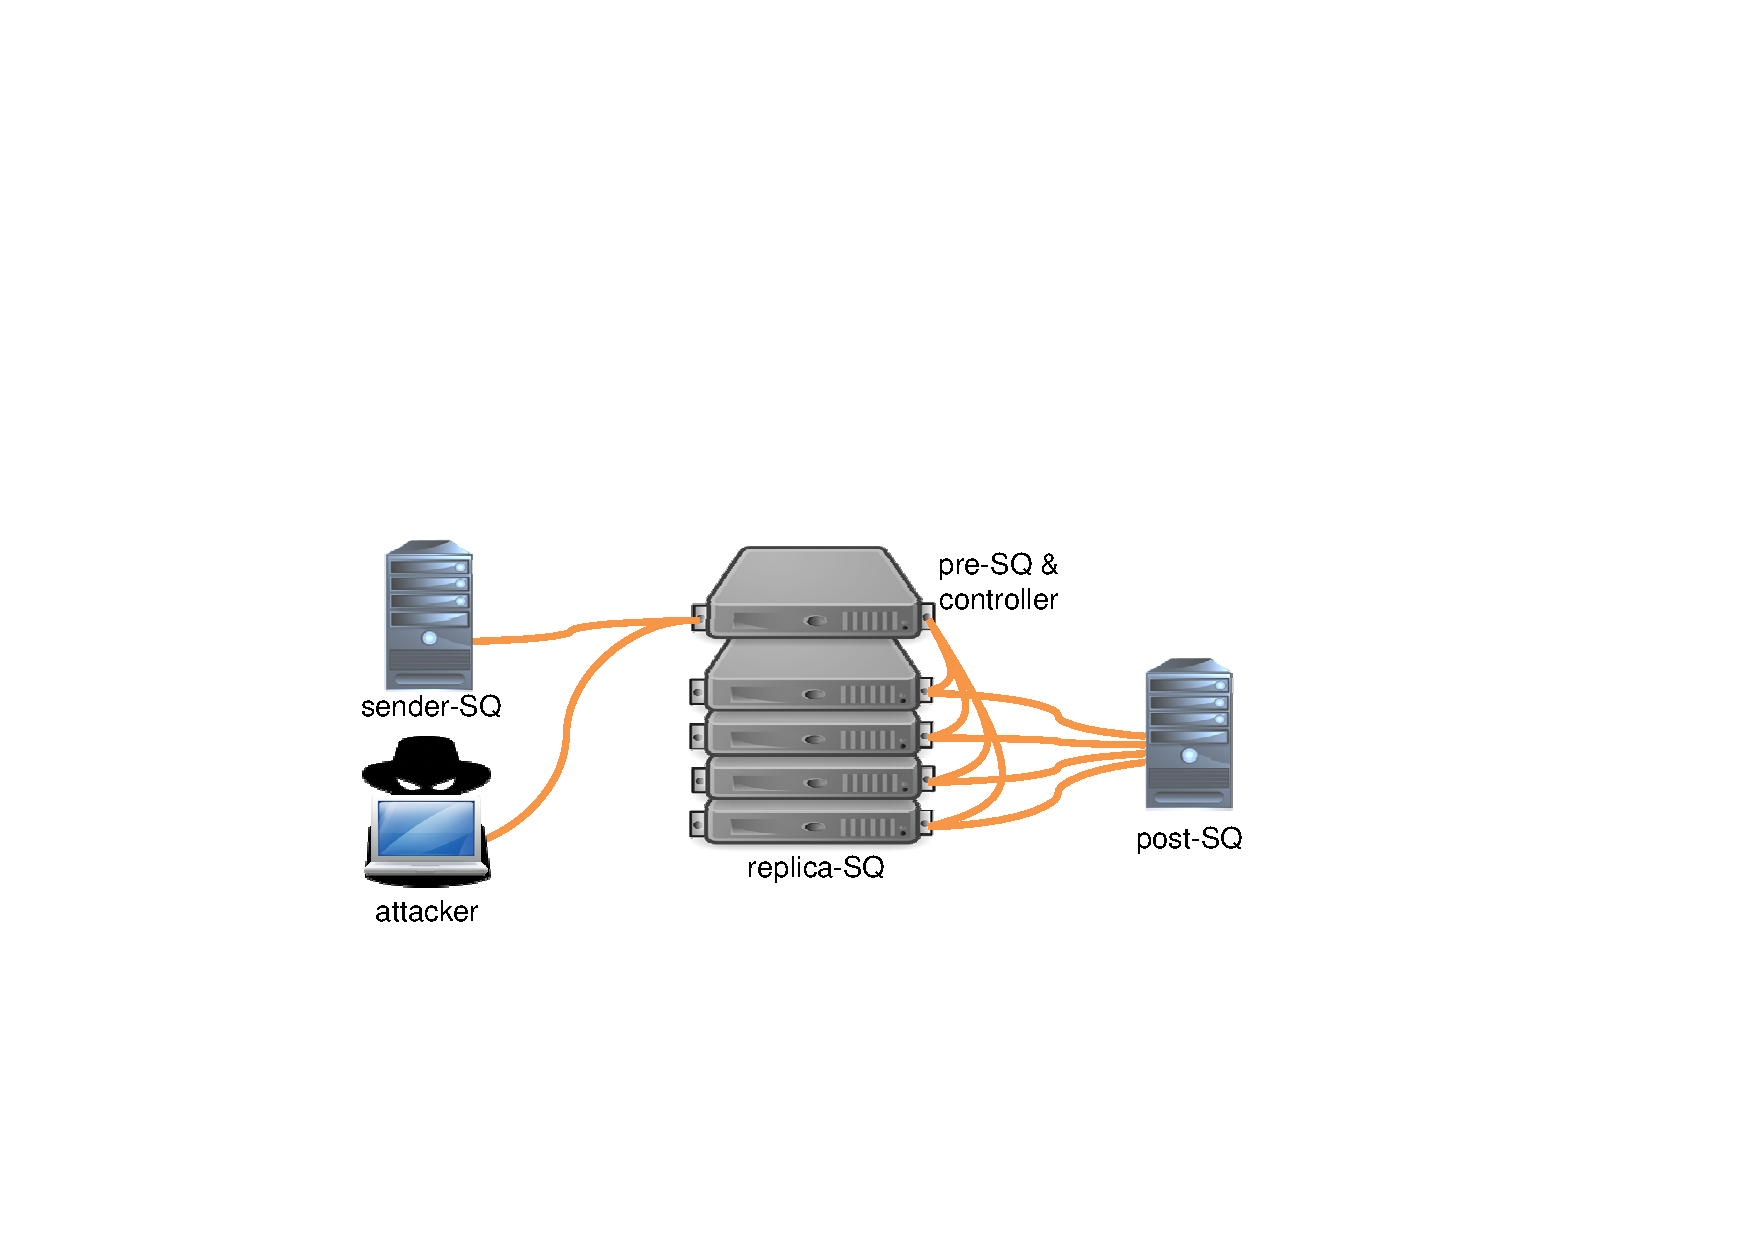
\includegraphics[width=0.8\columnwidth]{images/images/testbed1.pdf}
\caption{The \sieveq testbed architecture used in the experiments.}
\label{fig:testbed}
\end{figure}


\subsection{Methodology}

\sieveq acts as a highly resilient protection device, receiving messages on one side and forwarding them to the other side.
Therefore, the performance of \sieveq is assessed with latency/throughput measurements that can be attained under different network loads. 
In the experiments, the sender transmits data at a constant rate, i.e., 100 to 10000 messages per second, with three different message payload sizes, i.e., 100 bytes, 500 bytes and 1k bytes.
We used the Guava library~\cite{guava} to control the message sending rate.


\emph{Latency} measures the time it takes to transmit a message from \sender until it is delivered to the application on the \postsieve. 
The following procedure was employed to compute the latency: \sender obtains the local time before transmitting a message. 
When the message arrives and is ready to be delivered to the receiver application (after voting), the \postsieve returns an acknowledgment over a dedicated \gls{udp} channel.
The \Sender gets the current time again when the acknowledgment arrives. 
The latency of a message is the elapsed time calculated at \sender (receive time minus send time) subtracted by the average time it takes to transmit a \gls{udp} message from \postsieve to \sender.

\emph{Throughput} gives a measure of the number of messages per second that can be processed by \sieveq. 
It was calculated at the \postsieve using a counter. 
This counter is incremented every time a message is delivered to the receiver application, and the counter is reset to zero after one second. 
Consequently, the server can calculate the number of messages delivered in every second. The throughput is computed as the average value of the individual measurements collected over a period of time (in our case, 5 minutes after the steady state was reached).

In some experiments, we wanted to assess the behavior of \sieveq under a DoS attack. 
The attack was made using PyLoris~\cite{pyloris}, a tool built to exploit vulnerabilities on \gls{tcp} connection handling.
The tool implements the Slowloris attack method, which opens many \gls{tcp} connections and keeps them open.
The tool allows the user to define parameters like group size of attack threads, the maximum number of connections, and the time interval between connections among others.
In our setup, PyLoris was configured to perform an unlimited number of connections, with $0.1$ milliseconds between each connection.

In all experiments, measurements were taken only after the \gls{jvm} was warmed-up, and the disks were not used (all data is kept in memory).


\subsection{Performance in Failure-free Executions}
\label{throughput_latency}

This experiment measures the latency of \sieveq with several message sizes and distinct message transmission rates. 
It demonstrates the overall performance of \sieveq in different scenarios, gradually stressing the \postsieve side as the workload is slowly increased. 
Measurements were collected after the system reached a steady state. 
The experiments were repeated 10 times for every workload and the average result is reported.

\begin{figure}[h]
\centering
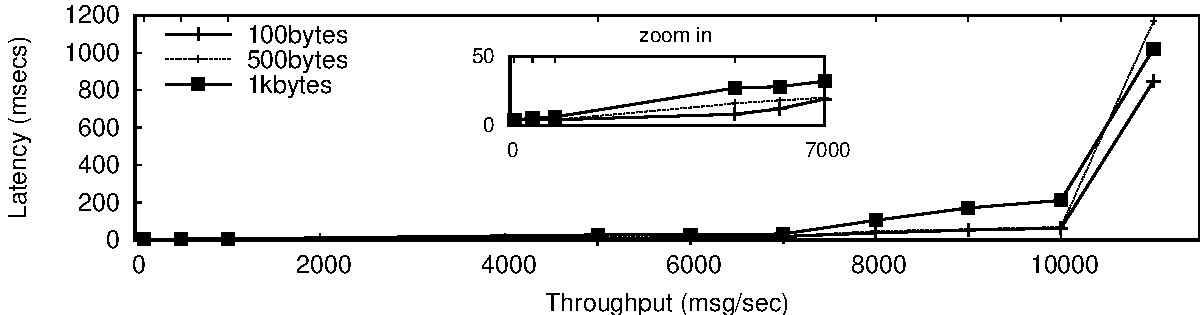
\includegraphics[width=\columnwidth]{images/gnuplot/sieveq/new_plot_latencyvsthroughput/latencyVSthroughput.pdf}
\caption{\sieveq latency for each workload (message size and transmission rate).}
\label{fig:lat_vs_throu}
\end{figure}

Figure~\ref{fig:lat_vs_throu} shows how the latency is affected by the transmission rate and message size.
As expected, when the system becomes increasingly loaded, the latency grows proportionally because resources have to be shared among the various messages.
The latency increase is approximately linear for the messages with 100 and 500 bytes until the throughput reaches $10k$ messages per second.
The messages with $1k$ bytes have a linear increase on latency until the throughput reaches approximately $7k$ messages per second, and then it has a higher increase as more load is put on the system.
This means that very high workloads can only be supported if applications have some tolerance to network delays.
Overall, the performance degrades gracefully when varying the message payload sizes, for rates under $7k$ messages per second.


\begin{table}[h]
\begin{center}
\begin{tabular}{c c c}\hline\hline
\textbf{Payload size } & \textbf{Non-optimized}  & \textbf{Optimized}   \\
\textbf{$(bytes)$} & \textbf{$(msg/sec)$} & \textbf{$(msg/sec)$}  \\\hline
$100  $ & 1360 & 10682 \\
$500  $ & 1320 & 10618 \\
$1000 $ & 1311 & 10332  \\
\hline\hline
\end{tabular}
\caption{Maximum load induced by the \sender library with various message sizes\label{tab:client_evaluation}}
\end{center}
\end{table}

We performed a more detailed analysis of the overheads introduced by the various components of \sieveq.
We observed that \sender performs the most expensive operations, which is interesting because it shows that our design offloads part of the effort to the edges, reducing bottlenecks.
%Nevertheless, the \sender library could still be optimized.
The most important overheads were caused by the tasks associated with securing the message payload (which in fact are the most costly operations in the system). Several optimizations were made to mitigate the performance penalties during the message serialization (e.g., creation of the signature), including the use of parallelization to take advantage of the multicore architecture (as done, for example, in~\cite{Kirsch:2014}).
Table~\ref{tab:client_evaluation} shows the gain of using the optimized version of the \sender library. Similar optimizations were employed in other components.



\subsection{Effect of Filtering Rules Complexity}

The results presented in the previous section do not consider any kind of complex filtering rule set.
This section presents experiments with a fully loaded system and application-level filtering rules with different complexity at the \repsieves.

Given the diverse requirements imposed by application-level firewalls, we decided to approximate the complexity of the filtering rules by considering a variable number of string matchings on processed messages.  It is well recognized that the most costly aspect of message filtering is exactly finding (or not) specific strings in the packet contents (besides crypto verifications, which were included in all our experiments). 
The high cost of running such algorithms leads for instance to several implementations in FPGAs and GPUs to improve performance in firewalls and \gls{ids} (e.g.,~\cite{Moscola:2003,Lee:2015}).

We used a classical algorithm for string matching (\gls{kmp}~\cite{Knuth:1977}) at the \repsieves to implement the filtering rules.
This algorithm is employed in \glspl{ids}~\cite{Prabha:2014} and firewalls like iptables~\cite{iptables}.
The algorithm employs a pre-computed table to execute string matching in $O(n + k)$ complexity, where $n$ is the string length and $k$ is the pattern length.


We measured the latency of the system by varying the message size from 100 to 1000 bytes and the string pattern size from 5 to 20 bytes. 
Both the message content and the strings were randomly generated. 
The experiments were performed with the maximum throughput of $10 000$ messages per second, as identified in the previous section. 
Figure~\ref{fig:KMP} shows the latency of \sieveq without message filtering (Baseline) and string matching (\gls{kmp}) with different sizes.
In the last group of experiments, where the message size is 1000 bytes and the pattern is 20 bytes, the latency increases by $50\%$. 
In other cases, sometimes higher overheads were observed, e.g., with 500 bytes messages and 20 bytes pattern the overhead is approximately $200\%$. 
This result is expected as the string matching is a slow operation and it needs to be performed in the critical path of message processing. 
Implementations with hardware support (as mentioned before) could be integrated with \sieveq to reduce these delays significantly.

\begin{figure}[!t]
\centering
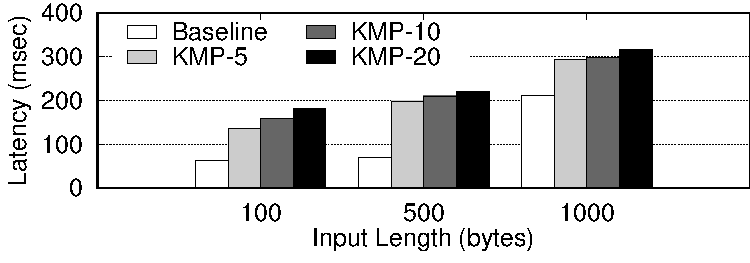
\includegraphics[width=\columnwidth]{images/gnuplot/sieveq/new_plot_fw/fw.pdf}
\caption{Comparison of the \sieveq's latency between the baseline and adding the filtering rules.}
\label{fig:KMP}
\end{figure}


\subsection{\sieveq Under Attack}

Our next set of experiments aims to evaluate the system under different attack scenarios.
Here, the \sender creates a steady load of 1000 500-byte messages per second.
We measured the latency and throughput of the system in three conditions: failure-free operation, a malicious external and internal DoS attack, and a malicious attack with remediation mechanisms.
%The results are reported in Figure~\ref{fig:performance_attacks}.
Before presenting the results, we need to stress that these experiments must be compared with the results displayed in Figure \ref{fig:attack_traditional}, which were obtained in the same way but with a different architecture (see Figure \ref{fig:traditional}).

Figure~\ref{fig:latency_normal} and Figure~\ref{fig:throughput_normal} show the latency and throughput, in the failure-free scenario.
One can observe that latency stays on average around $3.4$ milliseconds.
The throughput is approximately constant during the whole period.
It is possible to observe some momentary spikes in the latency and throughput, which happens due to Java garbage collector and a queuing effect from the \gls{smr}.

\begin{figure}[h]

\subfloat[Baseline latency.]{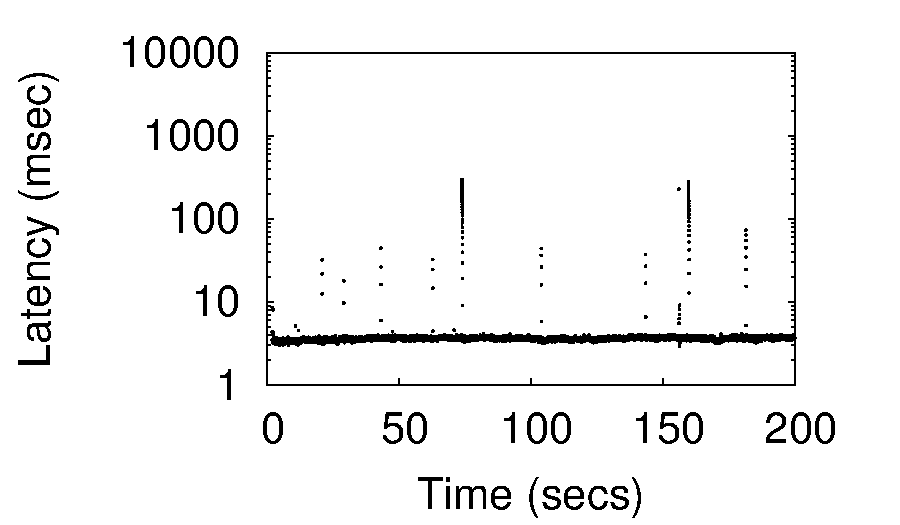
\includegraphics[width=0.5\columnwidth]{images/gnuplot/sieveq/plots/latency_normal_t1000_s500.pdf}\label{fig:latency_normal}}
\hspace{-5mm}
\subfloat[Baseline throughput.]{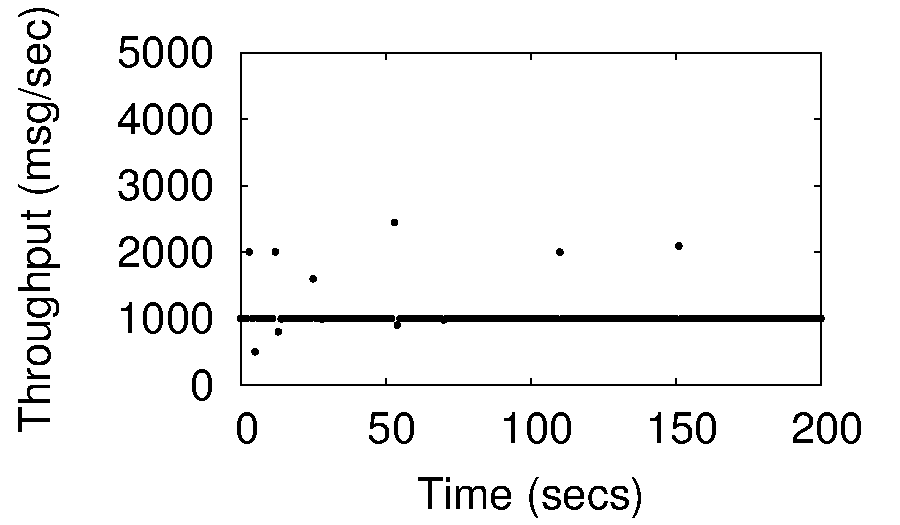
\includegraphics[width=0.5\columnwidth]{images/gnuplot/sieveq/plots/server_throughput_normal.pdf}\label{fig:throughput_normal}}
\caption{Performance of \sieveq under different attack conditions.}
\label{fig:performance_attacks}
\end{figure}



The behavior of the \sieveq during a \gls{dos} attack is displayed in Figure~\ref{fig:latency_attack} and Figure~\ref{fig:throughput_attack}.
In this scenario, we have disabled the \sieveq capability of replacing \presieves at runtime.
The attack consists in stressing the \gls{tcp} socket interface of the \presieves by creating many \gls{tcp} connections, which consumes network bandwidth and wastes resources at system and application levels. When the attack is started it executes for 50 seconds. The latency graph displays a reasonable impact in terms of an increase in the delays for message delivery. 
In some cases, the latency is not too affected but in others, there is a drastic delay, with some messages taking more than 3 seconds.
The attack also has consequences on the throughput as it is possible to observe an oscillation between 0 to 4000 messages per second (which correspond to the situation when the \postsieve processes a batch of messages that have been accumulated).

\begin{figure}[h]
\subfloat[DoS w/ no recovery.]{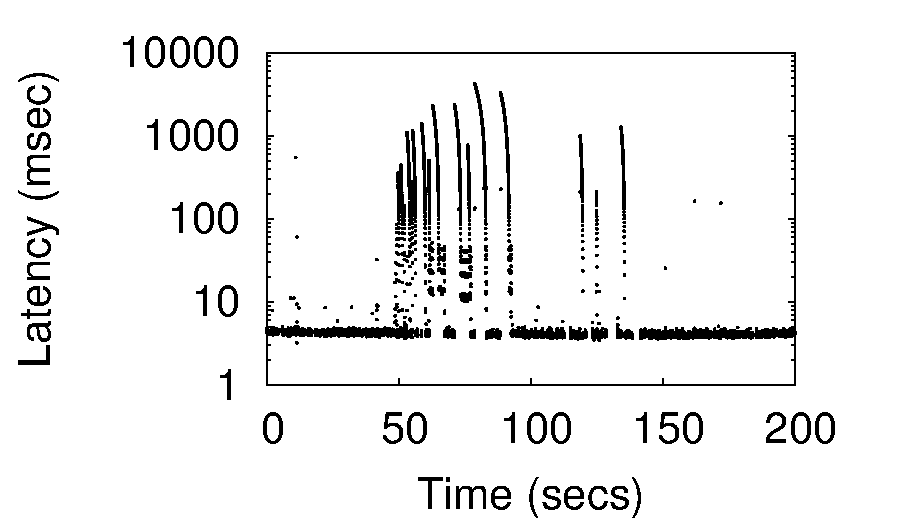
\includegraphics[width=0.5\columnwidth]{images/gnuplot/sieveq/plots/latency_normal_t1000_s500_under_attack.pdf}\label{fig:latency_attack}}
\hspace{-5mm}
\subfloat[DoS w/ no recovery.]{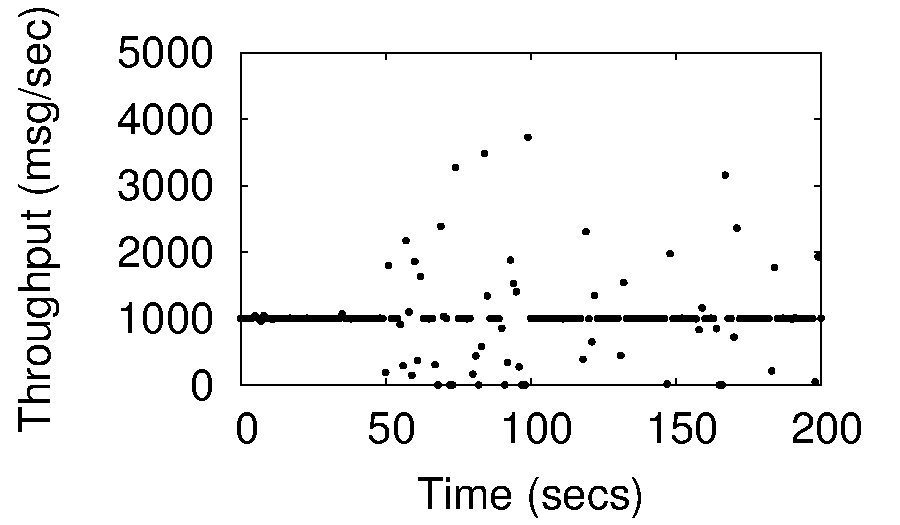
\includegraphics[width=0.5\columnwidth]{images/gnuplot/sieveq/plots/server_throughput_attack.pdf}\label{fig:throughput_attack}}
\hspace{-5mm}
\caption{Performance of \sieveq under different attack conditions.}
\label{fig:performance_attacks}
\end{figure}

Figure~\ref{fig:latency_attack_replacement} and Figure~\ref{fig:throughput_attack_replacement} show the latency and throughput when a similar \gls{dos} was carried out, but in this case the \sieveq replaced the \presieve under attack with a new \presieve.
When the \presieve finds out that it is being overloaded with messages coming from non-authorized senders, it asks for a replacement.
After that, the controller replaces the faulty \presieve, and the existing \senders are contacted to migrate their connections.
As the figures show, the impact of the attack is minimized, since only a few messages are delayed and throughput is only affected momentarily while the \presieve is switched.
Once the new \presieve takes over, the messages lost during the switching period are retransmitted and delivered.
In practice, the attack becomes ineffective because, although it continues to consume network bandwidth, there is no longer a \presieve to process the malicious messages.
An adversary could increase the attack sophistication and try to find a new \presieve target.
However, even in this case the attack has limited effect because during an interval of time (while there is a search for a fresh target) the system can make progress.

\begin{figure}[h]
\subfloat[DoS w/ recovery.]{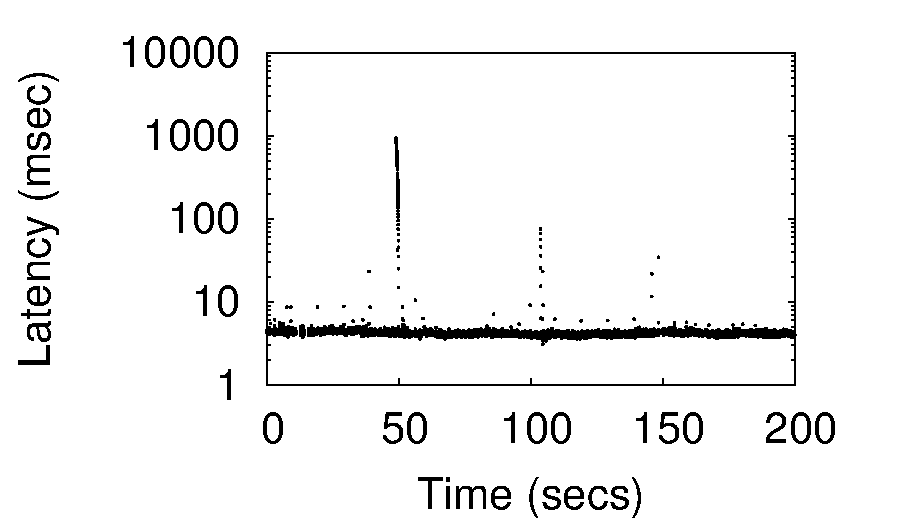
\includegraphics[width=0.5\columnwidth]{images/gnuplot/sieveq/plots/latency_t1000_s500_change_with_attack.pdf}\label{fig:latency_attack_replacement}}
\hspace{-5mm}
\subfloat[DoS w/ recovery.]{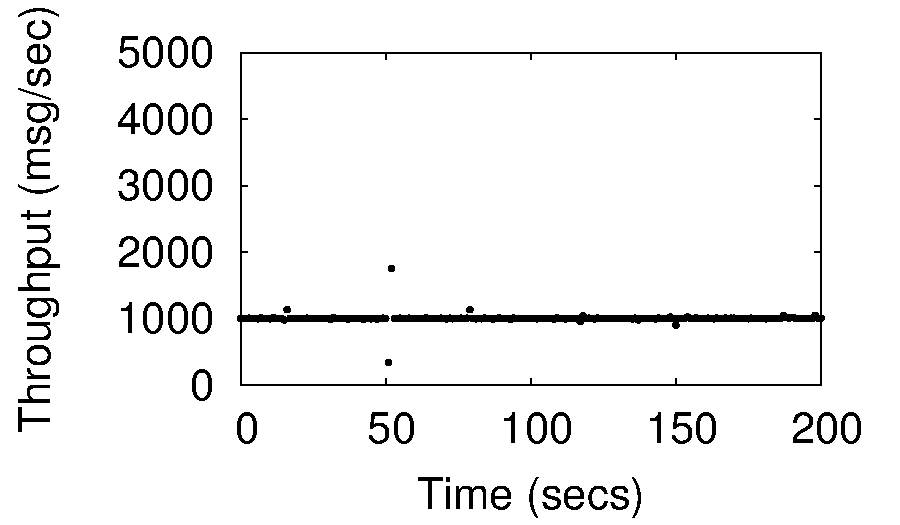
\includegraphics[width=0.5\columnwidth]{images/gnuplot/sieveq/plots/server_throughput_with_attack_change.pdf}\label{fig:throughput_attack_replacement}}
\hspace{-5mm}
\caption{\small Performance of \sieveq under different attack conditions.}
\label{fig:performance_attacks}
\end{figure}


Figure~\ref{fig:replica_dos_no_recovery} and Figure~\ref{fig:replica_dos_recovery} shows the \sieveq throughput when an internal attack is carried out by a compromised \repsieve. 
The experiment was made with a \repsieve ($r1$) launching a \gls{dos} to another \repsieve ($r2$).
The attack consists in overloading a \repsieve with \emph{state transfer} requests, which are the most demanding request a replica can receive in BFT-SMaRt~\cite{Bessani:2013}.
Figure~\ref{fig:replica_dos_no_recovery} shows the impact on the \sieveq throughput during an attack lasting 50 seconds, without any recovery capability on the system.
As can be seen, the performance of the system is severely disrupted during the attack.
Figure~\ref{fig:replica_dos_recovery} shows the same attack but with the detection and recovery mechanism described in Section~\ref{faultyrepsieve}.
The \postsieve detects the problem by noticing that $\mathit{f_{rs}+1}$ \repsieves are sending less messages than the others, and then requests a recovery.
When the \repsieve is recovered it requests the state from the other replicas, and then after applying the new state, the replica resumes the normal execution (end line in the figure).
In the experiment of Figure \ref{fig:replica_dos_recovery} we show a case in which the faulty \repsieve is the first to be recovered.
It could happen that \sieveq recovered $\mathit{f_{rs}}$ \repsieves before the faulty one.
This would take  $\mathit{(f_{rs}+1)} \times$ 3 seconds (in our setup) before the system resumes the normal execution.


\begin{figure}[h]
\subfloat[Internal DoS execution without recovery actions.]{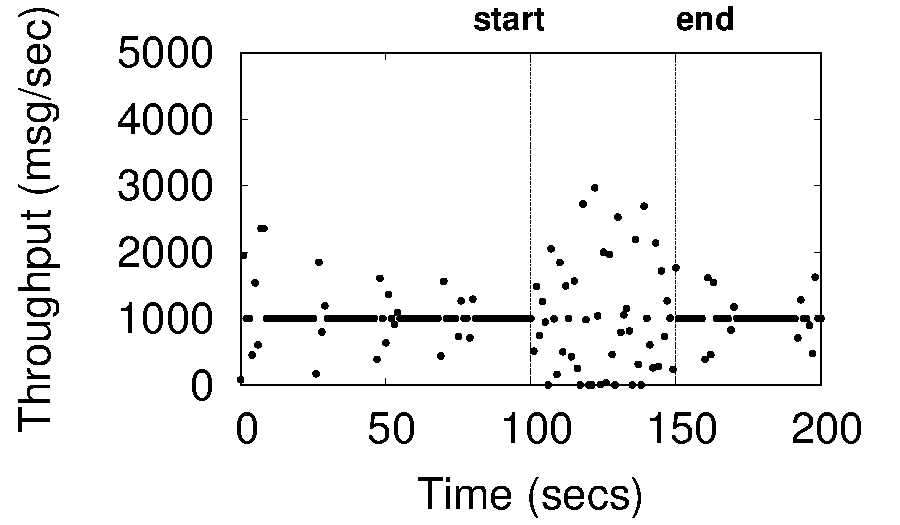
\includegraphics[width=.5\columnwidth]{images/gnuplot/sieveq/new_internal_recovery/server_throughput_no_recovery_replicas_dos.pdf}\label{fig:replica_dos_no_recovery}}
\subfloat[Internal DoS execution with recovery actions.]{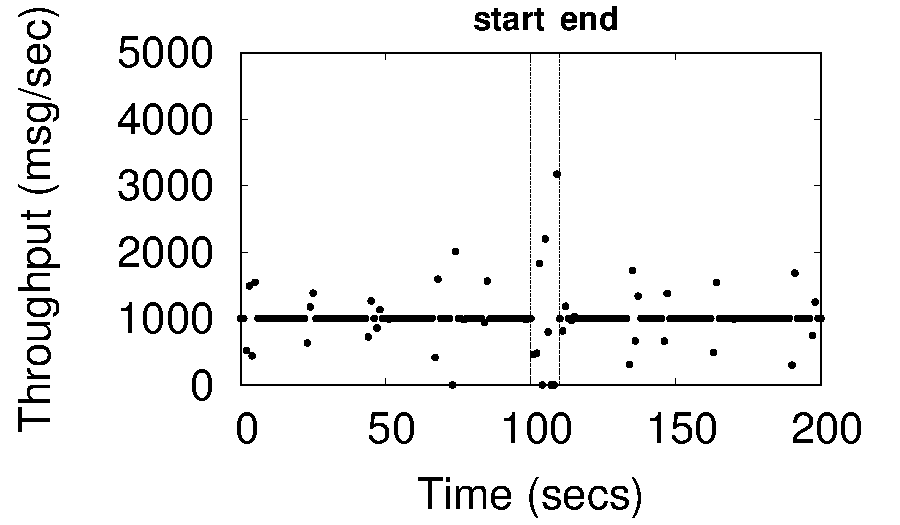
\includegraphics[width=0.5\columnwidth]{images/gnuplot/sieveq/new_internal_recovery/server_throughput_recovery_replicas_dos.pdf}\label{fig:replica_dos_recovery}}
\caption{Performance of \sieveq under different attack conditions.}
\label{fig:performance_attacks}
\end{figure}

\subsection{Use Case: \sieveq to Protect a SIEM System}
\label{use_case}

\gls{siem} systems offer various capabilities for the collection and analysis of security events and information in networked infrastructures~\cite{Miller:2010}.
These systems are being employed by organizations as a way to help with the monitoring and analysis of their infrastructures.
They integrate a large range of security and network capabilities, which allow the correlation of thousands of events and the reporting of attacks and intrusions in near real-time.

A \gls{siem} operates by collecting data from the monitored network and applications through a group of sensors, which then forward the events towards a correlation engine at the core facility.
The engine performs an analysis of the stream of events and generates alarms and other information for post-processing by other \gls{siem} components.
Examples of such components are an archival subsystem for the storage of data needed to support forensic investigations, or a communication subsystem to send alarms to the system administrators.

\begin{figure}[!h]
\centering
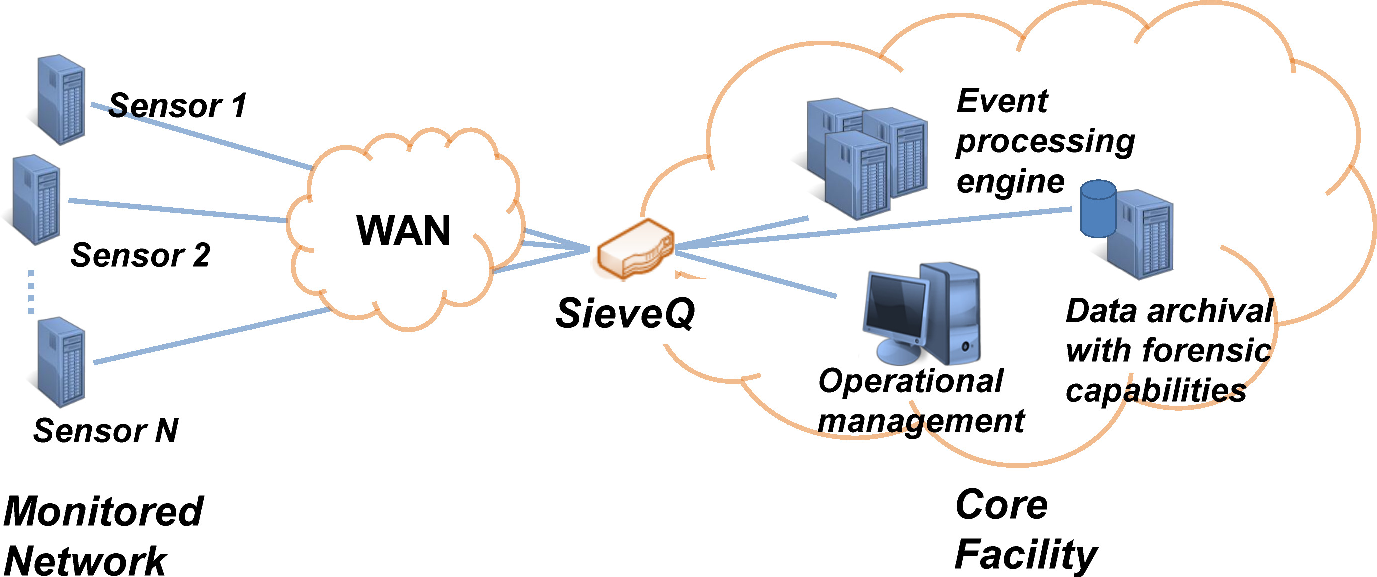
\includegraphics[width=0.65\columnwidth]{images/images/SIEM.pdf}
\caption{Overview of a SIEM architecture, showing some of the core facility subsystems protected by the \sieveq.}
\label{fig:siem}
\end{figure}

As part of the MASSIF European project~\cite{Vianello:2013}, we have implemented a resilient \gls{siem} system, where \sieveq was used to protect the access to the core facility (in Figure~\ref{fig:siem}).
In the \sieveq architecture, the sensors had the \sender while the \postsieve was placed in the correlation engine.
Additionally, we had access to an anonymized trace with the security events collected during the 2012 Olympic Games.
Each event corresponds basically to a string describing some observed problem by a sensor. The strings had lengths varying between a minimum of 551 bytes and a maximum of 2132 bytes, with an average length of 1990 bytes (and a standard deviation of 420 bytes). Based on this log, we built a sensor emulator that generates traffic at a pre-defined rate. Basically, when it is time to produce a new event, the emulator selects an event from the trace and feeds it to the \sender.

During the 2012 Olympic Games, the workload was approximately 11 million events per day, i.e., around 127 events per second.
Figure~\ref{fig:massif} shows the latency imposed by \sieveq for this workload, and when it is scaled up from 2 to 16 times more. 
As can be observed, the latency is in the order of 4 milliseconds for the emulated scenario.
Even with the highest load (16 times) the observed values had a latency below $70$ milliseconds.
This means that \sieveq could potentially deliver on average 176 million events per day, which is more than enough to accommodate the expected growth in the number of events for the next Olympic Games.

\begin{figure}[!h]
\centering
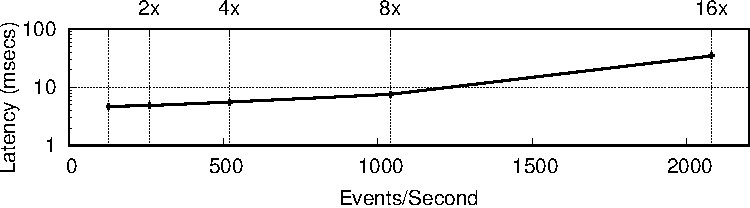
\includegraphics[width=\columnwidth]{images/gnuplot/sieveq/new_massif/massif.pdf}
\caption{\sieveq latency for the 2012 Summer Olympic Games scenario throughput requirement (127 events per second) and how the \sieveq scale, we doubled on each experiment the number of events.}
\label{fig:massif}
\end{figure}

\section{Discussion}
\label{discussion}

\sieveq differs from standard firewalls like iptables~\cite{iptables} that do not need client- or server-side code modifications.
However, our system requires these modifications to ensure end-to-end message integrity and tolerance of compromised components.
Complete transparency would be hard to achieve mainly due to the use of voting.
Nonetheless, it is worth stressing that \sieveq is to be used as an additional protection device in critical systems, not as a substitute to normal L3 firewalls.
\sieveq provides a protection similar to an application-level/L7 firewall, as one can implement arbitrary rules on the \repsieve module.


State machine replication is a well-known approach for replication~\cite{Schneider:1990}.
In this technique, every replica is required to process requests in a deterministic way.
This requirement traditionally implies in two limitations: (1) replicas cannot use their local clock during request processing; and (2) all requests are executed sequentially.
The first limitation can affect the capacity of \sieveq to process rules that use time.
We remove this limitation by making use of the timestamps generated by the leader replica and agreed upon on each consensus, as proposed in PBFT~\cite{Castro:2002} and implemented in BFT-SMaRt~\cite{Bessani:2014}.
The second limitation can constraint the performance of the system, especially when CPU-costly operations such as signature verifications are executed.
One of the optimizations we implemented in \sieveq was to add multi-threading support in the BFT-SMaRt replicas.
More precisely, the signature verification is done by a pool of threads that either accept or discard messages.
Once accepted, a message is added to a processing queue following the order established by the total order multicast protocol.
A single thread consumes messages from this queue, verifies them against the security policy, updates the firewall state (if needed) and forwards them to their destinations, without violating the determinism requirement.




\section{Final Remarks}
\label{sec:finalremarkssieveq}


We presented \sieveq, a new intrusion-tolerant protection system for critical services, such as \gls{ics} and \gls{siem} systems.
Our system exports a message queue interface which is used by senders and receivers to interact in a regulated way.
The main improvement of the \sieveq architecture, when compared with previous systems, is the separation of message filtering in several components that carry on verifications progressively more costly and complex.
This allows the proposed system to be more efficient than the state-of-the-art replicated firewalls under attack.
\sieveq also includes several resilience mechanisms that allow the creation, removal, and recovery of components in a dynamic way, to respond to evolving threats against the system effectively. 
Experimental results show that such resilience mechanisms can significantly reduce the effects of \gls{dos} attacks against the system.


